%-----CLASS LOADING-------------------
\ifx\pdfoutput\undefined
\documentclass[a4paper,twoside,12pt,dvips]{article}
\else
\documentclass[a4paper,twoside,12pt,pdftex]{article}
\fi

%-----INPUT ENCODING-----------------
\usepackage[utf8]{inputenc}

%-----LANGUAGE SELECTION-------------
\usepackage[english]{babel}

%-----PACKAGES SELECTION-------------
\usepackage{graphicx,color,hyperref,amsmath,fancyhdr,keystroke}
\usepackage{tabularx,multirow,rotating}

\graphicspath{{figures/}} 

%-----CONFIG HYPERREF-----------------
\definecolor{rltred}{rgb}{0.75,0,0}
\definecolor{rltgreen}{rgb}{0,0.25,0}
\definecolor{rltblue}{rgb}{0,0,0.75}
\hypersetup{colorlinks=true,
  urlcolor=rltblue,                % \href{...}{...} external (URL)
  filecolor=rltgreen,              % \href{...} local file
  linkcolor=rltred,                % \ref{...} and \pageref{...}
  citecolor=rltblue,               % \cite{}
  bookmarks         = true,        % Signets
  bookmarksnumbered = true,        % Signets numerotes
  pdfpagemode       = UseOutlines, % Signets/vignettes ferme a l'ouverture
  pdfstartview      = FitV,        % La page prend toute la largeur
  pdfpagelayout     = OneColumn,   % Vue par page
  pdfborder         = {0 0 0},     % Style de bordure : ici, pas de bordure
  pdftitle          = {XFLR5 v6.02 Guidelines},
  pdfauthor         = {},
  pdfsubject        = {XFLR5 v6.02 Guidelines},
  pdfkeywords       = {xflr5 guidelines}
}

%-----PAGE LAYOUT---------------------
% http://www.ctan.org/tex-archive/macros/latex/contrib/fancyhdr/fancyhdr.pdf
% http://amath.colorado.edu/documentation/LaTeX/reference/layout.html
% Lot of other ressources about Latex page layout on the web ...

%-header and footer-
\pagestyle{fancy}
\rhead[~]{~}
\chead[~]{~}
\lhead[{\small XFLR5 v6.02 Guidelines}]{~}
\lfoot[\textbf{\thepage}]{~}
\cfoot[~]{~}
\rfoot[\today]{ \textbf{\thepage} }
\renewcommand{\headrulewidth}{0.2pt}
\renewcommand{\footrulewidth}{0.2pt}

%-margins- A4 = 297 x 210 mm = 11.7 x 8.3 inches (1in~2.2cm)
\setlength{\hoffset}{0in}
\setlength{\oddsidemargin}{0in}
\setlength{\evensidemargin}{0in}
\setlength{\textwidth}{6.3in} % 6.3in (16cm) (1in on each side)
\setlength{\linewidth}{\textwidth}
\setlength{\headwidth}{\textwidth}

\setlength{\voffset}{-0.75in}
\setlength{\topmargin}{0in}
\setlength{\headheight}{0.5in}
\setlength{\headsep}{0.25in}
\setlength{\textheight}{9.7in} % 9.7in (22cm) (1in on the top and bottom)
\setlength{\footskip}{0.75in}

%-paragraphs
\setlength{\parindent}{0in}
%\renewcommand{\baselinestretch}{1.1}
%\setlength{\parskip}{0.2\baselineskip}

% 8<-----DOCUMENT------------------------

\begin{document}

% 8<---------------------------------------------------------------------------

\title{

\includegraphics[width=0.8\linewidth]{img-01}\\
Analysis of foils and wings\\
operating at low Reynolds numbers}
\author{}
\date{28/02/2013}

\maketitle

\clearpage

% 8<---------------------------------------------------------------------------

\tableofcontents

\clearpage

% 8<---------------------------------------------------------------------------

\section{Purpose}

This document is not intended as a formal help manual, but rather as
an aid in using XFLR5. Its purpose is to explain the methods used in
the calculations, and to provide assistance for the less intuitive
aspects of the software.

% 8<---------------------------------------------------------------------------

\section{Introduction}

\subsection{Code limitations and domain of validity}

Like the original XFoil, this project has been developed and released
in accordance with the principles of the GPL. Among other things, one
important point about GPL is that :

\begin{quotation}
This program is distributed in the hope that it will
be useful, but WITHOUT ANY WARRANTY; without even the implied warranty
of MERCHANTABILITY or FITNESS FOR A PARTICULAR PURPOSE. See the GNU
General Public License for more details.
\end{quotation}

The code has been intended and written exclusively for the design of
model sailplanes, for which it gives reasonable and consistent
results.  The code's use for all other purpose, especially for the
design of real size aircraft is strongly disapproved.

\subsection{XFLR5's development history}

The primary purposes for the development of XFLR5 were to provide :

\begin{itemize}
\item A user-friendly interface for XFoil
\item A translation of the original FORTRAN source code to the
C/C++ language, for all developers who might have a need for it
\end{itemize}

This was done in accordance with, and in the spirit of, Mark Drela's
and Harold Youngren's highly valuable work, which they have been kind
enough to provide free of use under the General Public License.

The resulting software is not intended as a professional product, and
thus it does not offer any guarantees of robustness, accuracy or
product support. It is merely a personal use application, developed as
a hobby, and provided under GPL rules for use by all.

For this reason, it should be noted and understood that XFLR5 may not
be default-free. Some significant bugs affecting result precision have
been reported in the beta releases and corrected.\newline
However, XFLR5 has been thoroughly tested against other software and
published experimental results, up to now with some success, and this
permits a limited amount of trust in the results it provides.

The algorithms for foil analysis implemented in XFLR5 are exactly the
same as those of the original XFoil code, except for the translation
from FORTRAN to C. No changes nor amendments have been made. The
translation in itself could have caused new bugs. However, the code
has been thoroughly tested against numerous original XFoil analyses,
always with consistent results. It may be found, in some cases, that
one of the two programs may not converge where the other will, or that
the path to convergence is different from one to the other. This is
due to the different manner in which floating point numbers and
calculations are processed by the two compilers. Having said this, the
converged results are always close, and any differences within the
convergence criteria set in the XFoil source code.\newline
Hence, both XFoil and XFLR5 results of airfoil analysis will be
referred to herein as "XFoil results".

Wing analysis capabilities have been added in version 2.00. Initially,
this was done at the suggestion of Matthieu Scherrer, who has
experimented with his Mathlab "Miarex" code the application of the
Non-linear Lifting Line Theory (herein referred to as "LLT") to the
design of wings operating at low Reynolds numbers.

Later on, the necessity arose to add the Vortex Lattice Method (herein
referred to as "VLM") for the design and analysis of wings with
geometries not consistent with the limitations of the LLT.

Version v3.00 introduced Katz and Plotkin's recommended VLM method
based on quadrilateral rings, and the VLM calculation of planes with
elevator and fin.

On March 31\textsuperscript{st}, 2007, XFLR5 has become an Open Source
Development Project hosted by Sourceforge.net.

Version v4.00 introduces a 3D panel method for wings and planes,
including modeling options for fuselages.

Up to this last version, XFLR5 has been developed specifically for
Windows, using Microsoft's MFC libraries. This is a limitation of the
product, making it non available for Unix, Linux, and MAC systems. It
has therefore been decided to re-write the code using the
cross-platform Qt4 libraries provided by Nokia. This version has been
released as XFLR5 v5. It does not offer any new functionality compared
to the original code.

Released in a beta version in September 2010, XFLR5 v6 introduces the
stability and control analysis, and a modification of the 3D-panel
method for the plane.

\subsection{Changes introduced in XFLR5 v6}

\subsubsection{Problem size}

The maximum acceptable size for mesh definitions has been increased from
2000 panels to 5000 panels max.

Since the memory allocation increases as the square power of the problem
size, this new version will reserve more memory at the program launch,
and may take longer to start on those computer with low RAM.

\subsubsection{Stability and control analysis}

"Control polars" have been replaced by "stability polars", with
evaluation of stability and control derivatives.

\subsubsection{Batch calculations}

It is now possible to run a batch calculations for a list of airfoils.

\subsubsection{3D panel method}

The 3D panel method is now processed differently for single wings and
for planes.

For the analysis of single wings, the full 3D method is available as
in v5, with the wings represented as thick surfaces with uniform
doublet and source distribution.

For planes, the full 3D method has been replaced in v6 by a mix
formulation of 3D panels for the fuselage, and thin surfaces for the
wings.

\subsubsection{Inertia estimations}

In the inertia evaluation of wings, the mass of each strip is
distributed along the strip proportionally to the foils thickness, and
is no longer concentrated at the quarter-chord position.

\subsection{Code structure}

Five different "Applications" have been implemented :
\begin{itemize}
\item Two direct design modes which are convenient to compare foils,
and to design new foils with the use of B-Splines
\item The mixed inverse (QDES) and the full inverse (MDES) foil design
routines, virtually unchanged from the original
\item The foil direct analysis routines (OPER)
\item The wing, plane and body design and analysis
\end{itemize}

\clearpage

% 8<---------------------------------------------------------------------------

\section{Foil Analysis and Design Modes}

\subsection{General}

This part of the code is built around XFoil and its main features,
i.e.  the design routines, and the direct and inverse analysis (OPER,
MDES, GDES, and QDES). Except for the implementation of the Windows
interface, no special feature has been added to these modules.

To run and use XFLR5, no special knowledge nor any previous experience
of XFoil is necessary, although users accustomed to XFoil should have
no difficulty in recognizing the new Windows-style menu options.

Since the analysis engine is very much unchanged from the original,
users are advised to refer to the original XFoil help to understand
the purpose, operation, and limitations of the foil direct and inverse
analysis. Their use in XFLR5 is basically the same, with a limited
number of necessary adaptations for the Windows interface.

\subsection{Direct Analysis [Oper]}

\subsubsection{Foil object}

\paragraph{Foil Database}

Foils are loaded from standard foil files and are stored in a runtime
database. Any number of foils may be loaded at any time.

\paragraph{File format}

XFLR5 recognizes only the plain traditional format for foils, i.e. files
which contain the foil's name on the first line,
followed by the X,Y coordinates, which run from the trailing edge,
round the leading edge, back to the trailing edge in either direction:

\begin{verbatim}
Foil Name
X(1) Y(1)
X(2) Y(2)
. .
. .
X(N) Y(N)
\end{verbatim}

All lines containing a \texttt{\#} character are ignored.\newline
No special checks are performed on the input geometry. Users are advised
to check the file format if the foil is not read properly by XFLR5.

\subsubsection{Foil Modification}

XFLR5 provides the same options for foil modification as the original
XFoil code. These are:

\begin{itemize}
\item local and global refinement
\item modification of the thickness, camber, max thickness and max
camber positions.
\end{itemize}

The modification of these parameters will cause a new foil to be
generated.

Whenever a foil is modified, deleted or overwritten, all its
associated results are deleted to ensure consistency.

Experience shows, and XFoil advises, that refinement of the foil's
panels, after it has been loaded or modified, is usually a prudent
measure to take before any analysis.

\subsubsection{Analysis/Polar object}

Unlike XFoil, an analysis of a given foil may be performed only after
a "polar object" has been defined and associated to this foil. The
results of the analysis will automatically be associated and added to
the polar object.

Any number of polars may be created and associated to a given foil.

A polar object is defined by:

\begin{itemize}
\item its Type
\item its Reynolds and Mach numbers
\item the laminar to turbulent transition criterion
\item the forced trip locations on top and bottom surfaces
\end{itemize}

By default, the transition number is set to 9, and the trip locations
are set at the trailing edge.

In addition to the Type 1, 2 and 3 polars which are unchanged from
XFoil, Type 4 polars have been introduced, showing data for a given
angle of attack at variable Re. The purpose is to enable determination
of the critical Re value.

\begin{figure}[htbp]
  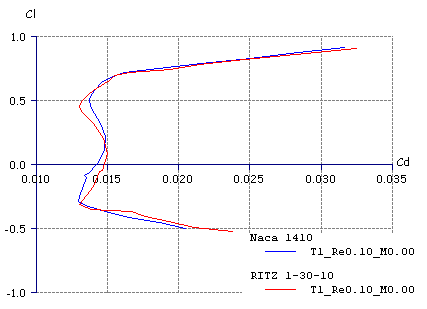
\includegraphics[width=0.8\linewidth]{img-02}\centering 
  \caption{Type 1 foil polars}
  \label{fig:type_1_foil_polars}
\end{figure}

\subsubsection{Operating Point (OpPoint) object}

An operating point of a given foil is defined by its angle of attack
and its Re number. Always associated to a foil and to a Polar object,
the OpPoint stores the inviscid and viscous results of the analysis.

Any number of OpPoints may be stored in the runtime database, the only
limitation being computer memory. OpPoints may use significant memory
resources.

To insure consistency, any modification to the foil or to the polar
causes the operating point to be deleted from the database.

\begin{figure}[htbp]
  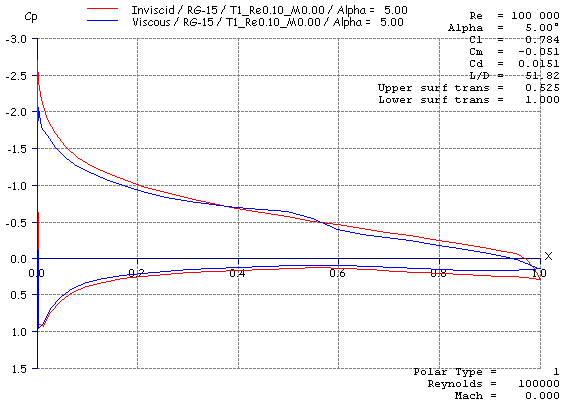
\includegraphics[width=0.8\linewidth]{img-03}\centering 
  \caption{$C_p$ calculation}
  \label{fig:c_p_calculation}
\end{figure}

\subsubsection{XFoil analysis}

Each time an XFoil direct analysis is performed and the convergence is
achieved, an OpPoint is generated and the values of interest are
stored in the currently selected polar object. Data is added to the
polar, whether the option to store OpPoints has been activated or not.

An XFoil calculation performed at the same angle of attack and Re as
an existing OpPoint causes the latter to be replaced, and the polar
data to be updated.

The "Init BL" checkbox is the equivalent of the "Init" menu
command in XFoil, i.e., it resets the boundary layer to standard
values before an analysis. It is recommended to check the box at the
time of the first calculation, and whenever the analysis of an OpPoint
is unconverged or is very different from the previous one.

In the case of sequential analysis, the "Init BL" is automatically
deactivated after a first converged point has been reached, and is
reset after an unconverged calculation.

\subsubsection{XFoil errors}

Given the complexity and difficulty of a viscous analysis, XFoil is
remarkably robust and consistent. It may happen however that the
following error message is generated during an analysis.

\begin{figure}[htbp]
  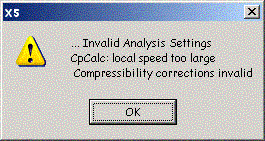
\includegraphics[width=0.4\linewidth]{img-04}\centering 
  \caption{XFoil Error Message}
  \label{fig:xfoil_error_message}
\end{figure}

This error message is usually caused by a too coarse paneling of the
foil, or a too sharp leading edge. It is possible that in such a case
XFoil gets "stuck" and fails at any attempt to perform a new
analysis. The menu command "Operating Point/Reset XFoil" can be used
to reinitialize all the variables and reset the currently selected
foils and polars.

\subsubsection{Session example Direct Analysis}

\begin{enumerate}
\item Load a foil from a file
\item (Optional) Use the "Derotate" and "Normalize" commands to
  respectively align the mean chord with the x-axis and to set its
  length to 1.
\item (Optional) Use the "Refine Locally" or "Refine Globally"
  commands to optimize the foil's panels
\item Use the "Define Analysis/Polar" command in the Polar menu, or
  \keystroke{F6}, to define an analysis -- for instance a Type 1 analysis at
  $Re \approx 100000$ and $Mach = 0.0$
\item Define an angle of attack or a lift coefficient to analyze --
  for instance $\alpha = 0^\circ$
\item Click on the "Analyze" button in the right toolbar to launch an
  analysis
\item If the XFoil analysis has converged, the $C_p$ distribution will be
  displayed automatically
\item Check the "Show BL" or "Show Pressure" buttons to visualize either
  distribution
\item Check the "Sequence" button in the right toolbar
\item Define the min and max angles for the analysis -- for instance
  from $\alpha = -6^\circ$ to $\alpha = 10^\circ$
\item Since the new start value is significantly different from the
  last calculation (i.e. $\alpha = 0^\circ$), check
  the "Init BLs" button
\item Click on the "Analyze" button
\item Click on the "Animate" button to visualize modifications of the
  boundary layer or pressure distributions with angle of attack
  variations
\item Click on the "Polars" command in the View menu, or type \keystroke{F8}
\item Use the mouse button and wheel to drag and zoom the graphs
\end{enumerate}

\subsection{Full Inverse Design [MDES] and Mixed Inverse Design [QDES]}

\subsubsection{General}

Both design modes are unchanged from the original.

Foils generated by the Full Inverse method are defined by 255
coordinate points, which is excessive for subsequent Direct
Analysis. A re-paneling of the foil is strongly recommended.

Although foils generated by the Mixed Inverse Method have the same
number of panels as the original foil, a re-panel is still advisable.

\subsubsection{Session example -- Full Inverse Design}

\begin{enumerate}
\item Switch to the Full Inverse Application (Menu command or \Ctrl +
\keystroke{3})
\item Select a foil from the loaded database, or load a foil from a
file
\item Click on the "New Spline" button in the right toolbar dialog
\item Select two points either on the upper or lower surface, but not
one on each
\item Drag the spline's control points to define a new speed
distribution
\item Click on the "Apply" button to register the change
\item Click on the "Execute" button to calculate the new foil
geometry
\item Use the mouse buttons and wheel to drag and zoom the graph and
the foil
\item Repeat the process until the desired geometry is reached
\item To store the modified foil, click on the arrow in the top
toolbar, or select "Store foil in the database" in the Foil menu
\item Switch to the Direct Analysis Application (Menu or \Ctrl +
\keystroke{5})
\item Use "Refine globally" in the Design menu to generate a coarser
panel
\item Proceed with the direct analysis
\end{enumerate}

\subsubsection{Session example -- Mixed Inverse Design}

Steps 1 to 6 are identical to the Full Inverse design method

\begin{enumerate}
\setcounter{enumi}{6}
\item Click on the "Mark for Modification" button to define which
part of the foil is to be modified
\item Click on the "Execute" button to calculate the new foil
geometry
\item Check for convergence in the text window\newline
In the case of non-convergence, it is possible either to resume
iterations by clicking again the "Execute" button, or to export the
modified geometry as it is
\end{enumerate}

Finish as with the Full Inverse design method.

\subsection{Foil Direct Design}

\subsubsection{General}

A crude design module has been included in XFLR5, which allows the
design of Foils either from B-Splines or from "Splined Points". The
former gives smoother surfaces, the latter authorizes greater control
over the geometry.

This design mode however is not the best way to design foils, and the
other possibilities derived from XFoil are far more adapted and
recommended i.e. :

\begin{itemize}
\item modification of a foil's thickness and camber
\item interpolation of foils
\item inverse methods
\end{itemize}

This foil design mode, however, may be useful to overlay different
foils and compare their geometries.

An option has been added in v6 to load a background image, with the
idea of digitalizing existing foils.

\subsubsection{B-splines main features}

Upper and lower surfaces are each determined by a separate and single
B-Spline.

Spline degree can be set between 2 and 5.

\subsubsection{Spline Points main features}

Upper and lower surfaces are each determined by a set of control points

Control points are linked by 3rd degree B-Splines

Two intermediate control points are added to the link splines, at 1/3
and 2/3 respectively of the separation of the two control
points. These two points are added automatically and are not visible,
nor can they be modified.

The slope at each visible control point is determined by the line
passing through the immediately previous and next control points.

\subsubsection{Leading and trailing edge}

For both methods, the slope at the leading edge is vertical and may
not be changed. In the case of a design from B-Splines, this is done
by forcing the second control point to remain on the vertical axis.
\newline
In the case of "Splined Points" the slope at the trailing edge is
determined by the position of two supplementary rear points, one for
each surface.

\subsubsection{Output precision}

The maximum number of output points on each surface is 150. This is
consistent with the sizing of the XFoil arrays, and with the precision
required for the application, although the increase of computing power
and memory capacity of modern computers could allow for more points.
Typically, XFoil requires at least 50 points on each side to perform
an adequate analysis.\newline
In both cases, it is prudent to "re-panel" the foil in the main
menu, to improve the convergence of the XFoil analysis and its
precision. This can be done with the equivalent of XFoil's "PANE"
and "CADD" commands. \newline
Upon exit from the design module, the user is asked whether to export
or not the foil to the analysis module.

\subsubsection{Digitalization}

An option has been added in v6.02 to load a background image. The
purpose is to enable digitialization of existing foil images using
splines.

After digitalization, the splines should be stored as a foil in the
database, and the foil ought to be normalized, de-rotated and
re-paneled.

\section{3D Analysis}

\subsection{Wind and body axis, sign conventions}

\begin{figure}[htbp]
  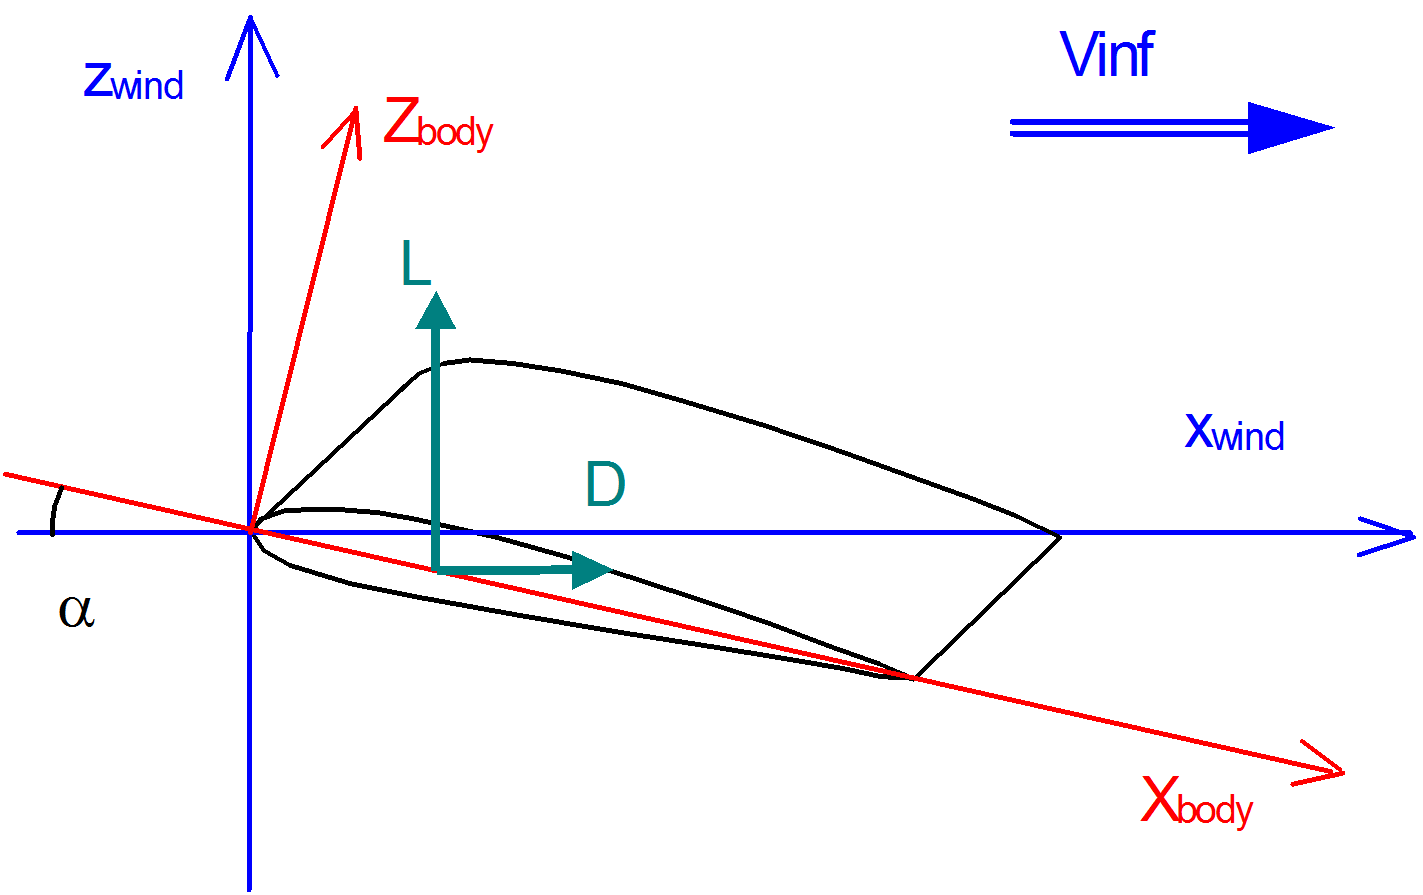
\includegraphics[width=0.8\linewidth]{img-05}\centering 
  \caption{Wind and Body axis}
  \label{fig:wind_and_body_axis}
\end{figure}

The lift and drag coefficients are given in wind axis.

\underline{Notes} 

\begin{itemize}
\item Up to v3.21, calculations have been performed using a small
angles approximation, which means that the wind and body axis were the
same.
\item Sign Conventions for moments -- Quote from Wikipedia, Flight
Dynamics :
\begin{quotation}
The most common aeronautical convention defines the roll as acting
about the longitudinal axis, positive with the starboard wing
down. The yaw is about the vertical body axis, positive with the nose
to starboard. Pitch is about an axis perpendicular to the longitudinal
plane of symmetry, positive nose up.
\end{quotation}
\end{itemize}

This is illustrated in the Figure~\ref{fig:moment_sign_convention}.

\begin{figure}[htbp]
  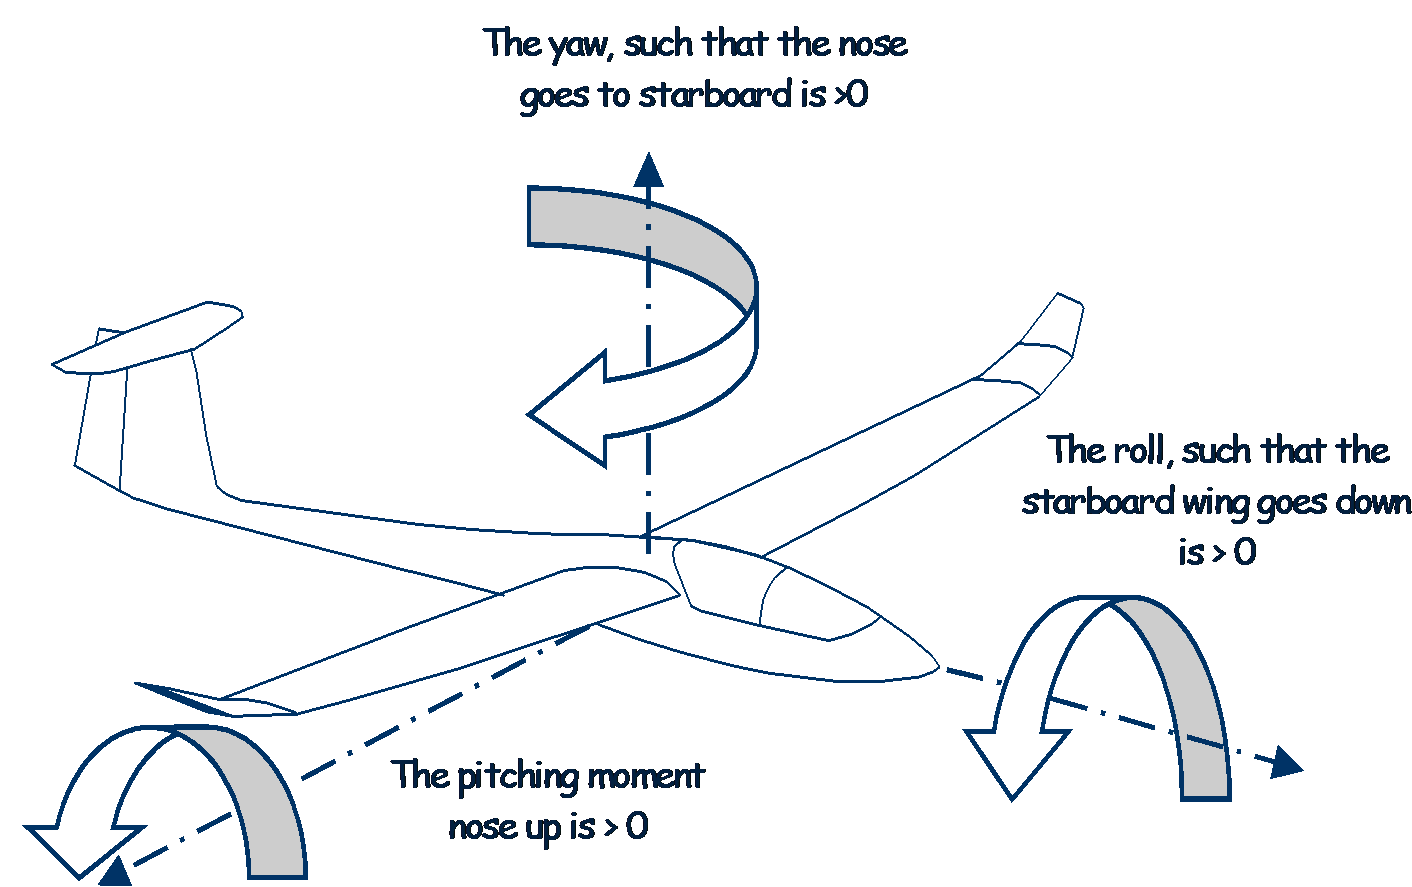
\includegraphics[width=0.8\linewidth]{img-06}\centering 
  \caption{Moment sign convention}
  \label{fig:moment_sign_convention}
\end{figure}

\subsection{Object Definition}

\subsubsection{Wing Definition}

\begin{figure}[htbp]
  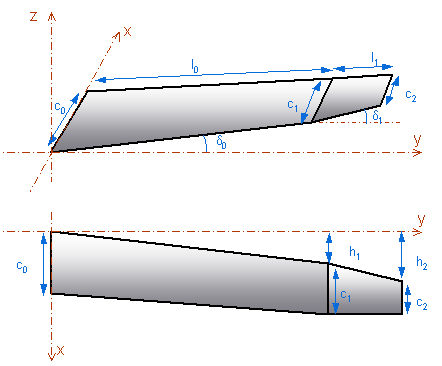
\includegraphics[width=0.8\linewidth]{img-07}\centering 
  \caption{Wing Definition}
  \label{fig:wing_definition}
\end{figure}

The wing is defined as a set of panels. Each panel is defined by :

\begin{itemize}
\item its length $l_i$,
\item the root and tip chords $c_i$ and $c_{i+1}$,
\item the leading edge offset at root and tip chords $h_i$ and
$h_{i+1}$,
\item the dihedral angle $\delta_\iota$,
\item the mesh for VLM analysis.
\end{itemize}

The spanwise length of a panel should be at least equal to the minimum
length of the VLM elements on other panels. Divisions by zero or
non-physical results could result from panels of insufficient length.

Twist (washout) is processed in LLT as a modification of the angle of
attack.

In VLM, the twist is processed as a modification of the wing, with the
rotation center located at the quarter chord point.\newline
Up to v3.04, the twist has been applied as a rotation of the sections
with respect to the absolute y axis. From v 3.05 onwards, the sections
are rotated with respect to the panel's quarter chord, i.e., after the
panel has been rotated by the dihedral angle. The results are impacted
for wings with panels well off the x-y plane.

The 'span' of the wing is defined as \[S = 2 \times \sum l_i\]

For ease of interpretation, the wing is shown developed on a horizontal
planform, both in the wing design dialog box and in the 2D view. Only
the 3D view gives a realistic representation of the geometry.

A wing may be asymmetric if the foils are different on each side. This
option is meant to provide some capability to evaluate the influence of
flaps, but should be used with caution. It has been tested neither
against experimental nor theoretical results.

\subsubsection{Reference area for aerodynamic coefficients}

The reference area for all wing and plane aerodynamic coefficients is
the main wing's area.

In the case of a bi-plane, the reference area is also the main wing's
area.

There reference lengths for moment coefficients are defined in
\S\ref{sec:moments}.

\underline{Notes} :

\begin{itemize}
\item Up to v.4.15, the reference area and the reference span have
been defined as the planform's area and span. With this convention,
the winglets' contribution are counted in the area and in the
span. This is not necessarily the best choice, since it is usually
convenient to compare performance coefficients of a wing with and
without winglets, but with a constant reference area.
\item Starting in v4.16, the default option is to use the planform
area and span projected on the xy plane. With this definition, the
contribution of the winglets to span and area is zero. For
convenience, it is still possible to choose either reference area; the
option can be set in the dialog box for analysis definition.
\end{itemize}

\subsubsection{Flaps}

From version v3.16 onwards, the automatic mesh methods takes into
account the breaks at the flap position, if both foils at each end of
the wing panel are defined with a flap.

The recommended way to create a flap is to define two foils at the same
spanwise position, the first with a flap break, the other without. The
code will ignore the zero-length panel.

\begin{figure}[htbp]
  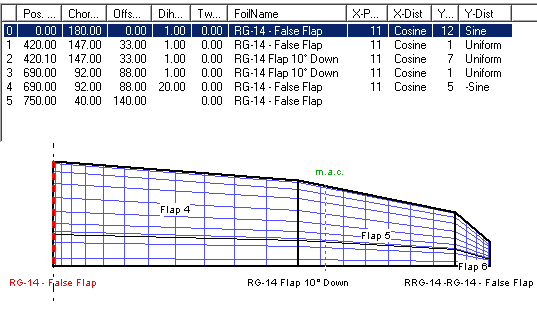
\includegraphics[width=0.8\linewidth]{img-08}\centering 
  \caption{Flap Definition}
  \label{fig:flap_definition}
\end{figure}

Triangular flaps, defined by a plain foil at one side of the panel and
by a flap break at the other side, are not recognized.

The flaps are counted as one for each wing side, e.g. ailerons are
counted as two flaps. This is necessary to calculate separately hinge
moments for asymmetrical wings.

\subsubsection{Body Design}

The modeling of the body is natural in a 3D panel method, but isn't
either without difficulties.

\paragraph{Modeling options}

Two options are provided, for two different purposes :

\begin{enumerate}
\item Representation by flat panels : this is the "Analysis"
purpose. \newline
Given an existing body, the idea is to digitalize its geometry and
input it in XFLR5. The resulting geometry will not be smooth, but it
is usually enough for prediction pruposes
\item Representation by B-Splines : this is the "Design"
purpose. \newline
The idea is to define and optimize a body geometry to achieve some
targeted aerodynamic (or cosmetic) performance. The body points can
then be exported to a text file for further use.
\end{enumerate}

\paragraph{Import/export of body data}

To facilitate the edition process, the control points can be edited in
a text file and imported in XFLR5, rather than being defined directly
in XFLR5.

An example of the format of the input file can be obtained by
exporting any existing body definition.

A typical format is :

\begin{verbatim}
Body_Name
...
FRAME
x_1 y_2 z_1
...
x_n y_n z_n

OFFSET
X_o Y_o Z_o

BODYTYPE
1 or 2
\end{verbatim}

\underline{Notes} :

\begin{itemize}
\item The keywords should be preceded by the character '\#'.
\item n is the number of side point definining the frame. This number
must be the same for all frame. If the frames are defined with
different numbers of points, the frame last defined will set the
number of points.
\item The frames are sorted by x positions
\item The points in the frame should be defined in clockwise order, on
the body's left side, when looking at the body from the front; this is
the view which is displayed in the right panel in the body design
module.
\item All points in a frame should have the same axial position
\item The x position of a frame is defined by the first point
\end{itemize}

\subsubsection{Plane Definition}

A plane consists in a main wing, and optionally of a secondary wing,
an elevator, one or two fins, and a body.

The body may be described either by cross-sections located at
different streamwise locations or by NURBS surfaces.

\paragraph[Surface assemblies]{Surface assemblies}

The main difficulty with the construction of a 3D plane model is to
connect the wing, elevator, fin and body together. Without the help of
a CAD system, it has been difficult to implement a versatile and
robust algorithm, mainly because of the number of configurations to
consider.  For instance, the elevator may or may not intersect the
body, it may or may not intersect the fin, it may intersect the body
only on its bottom or upper surface, etc.

The only surface verification implemented in V4.00 is a trim of the
wings, elevator and fin to the body's surface, and even then, the
algorithm may not be robust for all configurations.

What's more, even if the wings, elevator and fin are trimmed to the
fuselage surface, the body's panels are not adapted to follow their
contour. This implies that some of the body's panels will be located
inside the volume, which is not consistent with the panel theory.

\paragraph{Tip Patches}

The Panel Theory requires that the volume on which the analysis is
performed is completely closed by the surfaces which support the
panels. In other words, a body or a wing cannot have an open end, in
which case a numerical error will occur.

To try to close the volumes, the code will automatically create tip
patches in the following cases :

\begin{itemize}
\item Left tip of the left wing, and right tip of the right wing
\item Top and bottom tips of fins
\end{itemize}

It will not create patches in the following cases :

\begin{itemize}
\item Gap at the center of the wing, i.e. if the first chord is
located at a positive span position
\item Junction of the wing and fuselage
\end{itemize}

\underline{Note} : the influence of these modeling errors on the results
is unknown.

\subsubsection{Inertia estimations}

A calculation form is available to provide an approximate evaluation
for the CoG position and for the inertia tensor associated to the
geometry.  The evaluation should not be understood as anything else
than a rough order of magnitude.

The inertia is evaluated in the default coordinate system, i.e. with
respect to the CoG. The tensor in other systems can be computed by the
appropriate tensor transformations.

The evaluation is based on the following assumptions.

\begin{itemize}
\item For the body, the mass is distributed uniformly in the external
surface, and this surface is assumed to have a uniform thickness. The
body is divided in $N_b$ elementary sections along the x-axis. The
weight is concentrated at the center of the cross section. This is
illustrated in Figure~\ref{fig:mass_representation_for_the_body}.
\item For the wings, the mass is assumed to be distributed uniformly
in the wing volume along the span.\newline
In XFLR5 v5, it has been modeled as point masses concentrated at the
quarter-chord point of distributed sections along the span.\newline
In XFLR5 v6, it is modeled as point masses distributed both in the
span and chord directions, as illustrated in
Figure~\ref{fig:mass_representation_for_the_wing}.
\item The mass distribution is independent of the wing's mesh used for
aerodynamic calculations
\item Parts such as actuators, battery, lead, or receiver should be
modeled separately as point masses.
\end{itemize}

\underline{Notes} :

\begin{itemize}
\item At this stage of the code development, the results are not used
at any point in the performance calculations. The inertia evaluations
are provided as a convenience for external stability analysis to be
performed with codes such as AVL.
\item The mass defined for wings and bodies is not the one used for
Type 2 calculations. The mass for type 2 is defined with the
Analysis/Polar.
\end{itemize}

\begin{figure}[htbp]
  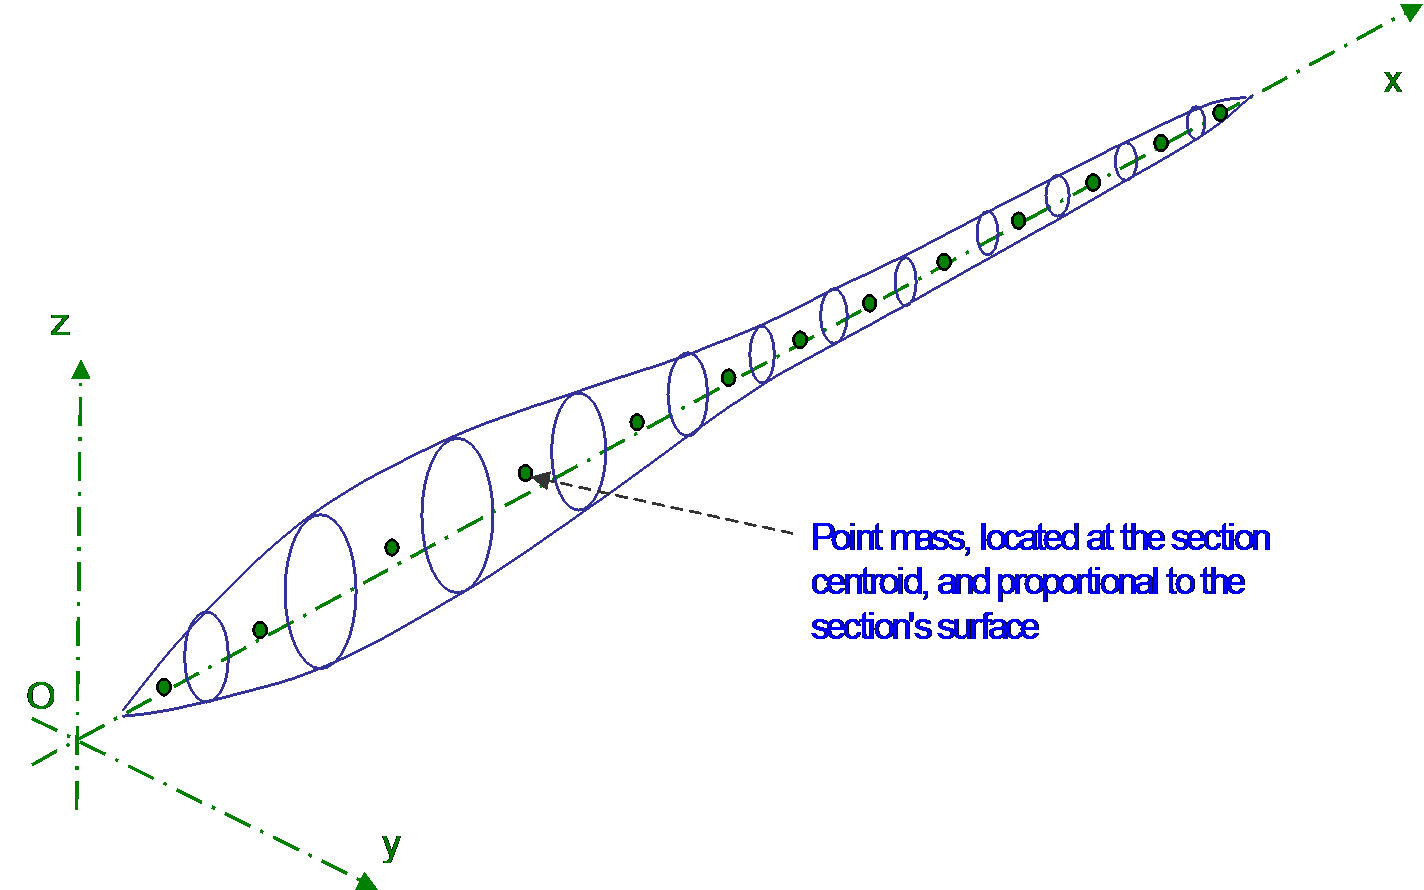
\includegraphics[width=0.8\linewidth]{img-09}\centering 
  \caption{Mass representation for the body}
  \label{fig:mass_representation_for_the_body}
\end{figure}

\begin{figure}[htbp]
  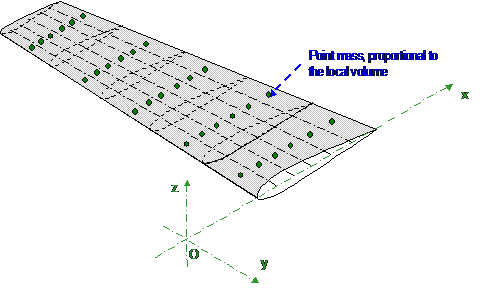
\includegraphics[width=0.8\linewidth]{img-10}\centering 
  \caption{Mass representation for the wing}
  \label{fig:mass_representation_for_the_wing}
\end{figure}


\subsubsection{Mesh}

The wing is "meshed" into a number of panels distributed over the
span and the chord of the planform, and a vortex or a doublet and
source is associated to each panel.

\begin{itemize}
\item The analysis may be of the VLM type and is performed on the mean
camber line
\item The analysis may be of the 3D-panel type in which case the wing
is modeled as a thick surface
\end{itemize}

It is recommended to choose a panel distribution which is consistent
with the wing's geometry, i.e. the density of the mesh needs to be
increased at geometrical breakpoints and at the root and tip of the
wings. A cosine type distribution is recommended in the chordwise
direction to provide increased density at the leading and trailing
edges.

There is a lower limit size for the panels below which the calculation
becomes unstable, or which leads to non-physical results. This can
typically occur with "sine" spanwise distributions of
panels. Ideally, the precision of the calculation increases with the
mesh's refinement, but so do the calculation times. It is fairly
simple to experiment to determine what is the best compromise for a
given design objective.

Numerical instability may also occur in 3D Panel analysis if a panel's
lengths in the streamwise and chordwise directions are too
different. The panel's aspect ratio should be kept low.

It is possible to exclude from the calculations the wing panels with a
spanwise length less than a minimum value. This can be set in the
advanced settings dialog box. If the minimum length is set to zero,
then all wing panels with length less than 1/1000 of the span will be
excluded. This is meant to avoid numerical errors linked to small mesh
elements.

Panel Methods :

\begin{enumerate}
\item The current implementation uses flat 1\textsuperscript{st} order
panels.\newline 
Ideally, these kind of panels need to have their four corners in the
same plane, which is not possible for twisted geometries. However,
this is not seen as a major issue for the low washout angles used for
model sailplane wings.
\item The surface velocity is the gradient of the doublet strengths
between adjacent panels as described in \cite{Maskew}. It is therefore
recommended to have the same number of chordwise panels along the
span, and the same type of distribution, either uniform or
sine.\newline 
Ideally, the panels should share the same edges and corner nodes. In
the case of a flap, the 'trick' to connect properly the panels is to
define a foil with a false flap set at $0^\circ$ flap angle, as is
illustrated in Figure~\ref{fig:mesh_disposition_for_a_flap}.
\end{enumerate}

\begin{figure}[htbp]
  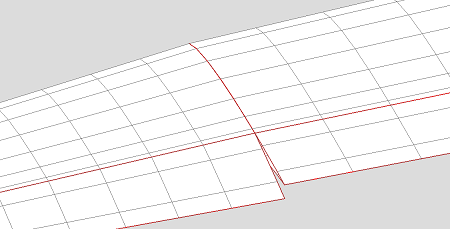
\includegraphics[width=0.8\linewidth]{img-11}\centering 
  \caption{Mesh disposition for a flap}
  \label{fig:mesh_disposition_for_a_flap}
\end{figure}

\paragraph{Panel arrangement - VLM analysis}

\begin{figure}[htbp]
  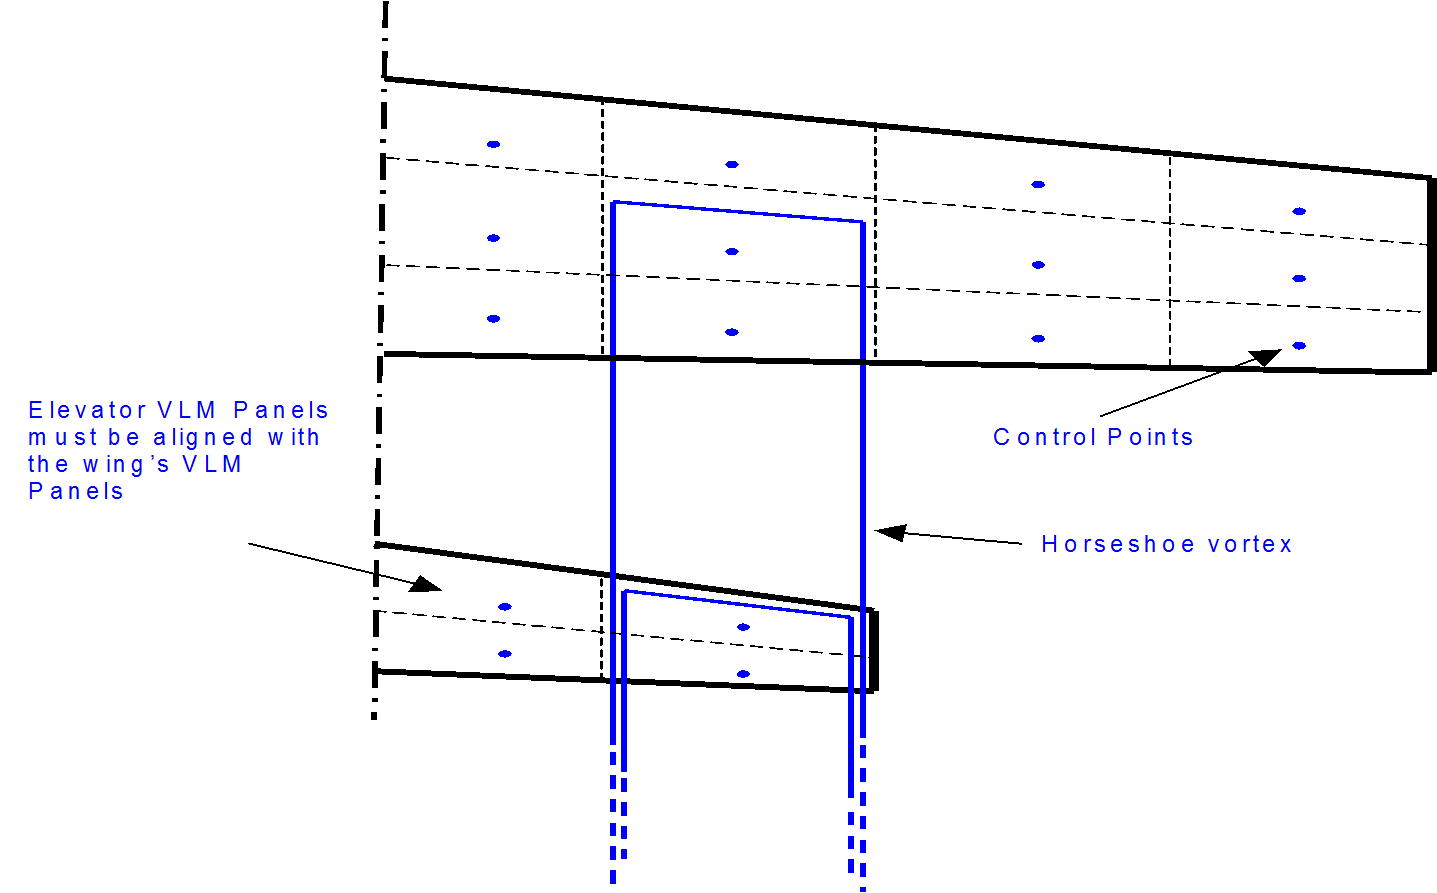
\includegraphics[width=0.8\linewidth]{img-12}\centering 
  \caption{VLM Panel arrangement for a plane}
  \label{fig:vlm_panel_arrangement_for_a_plane}
\end{figure}

Special care must be taken in the disposition of VLM panels to avoid
having a control point of the tail's surface close to the trailing leg
of one of the wing's horseshoe vortex.  This would lead to a division
by zero, and inconsistent results.

One method to avoid this issue is to have the wing's panels aligned
with those of the elevator.

For the same reason, it is a good idea, though not compulsory, to
position fins in the planes of the wing's panel junctions.

\paragraph{Panel arrangement - 3D panel analysis}

\subparagraph{Chordwise panels}

The Cp distribution is calculated as the derivative of the doublet
strength along the panel chordwise and spanwise strips.To achieve this,
it is required that each wing has a uniform number of chordwise mesh
panels along the span. It is also recommended that the chordwise panel
distribution be the same from one wing panel to the next, i.e. cosine
distribution for each wing panel. This is necessary to connect
adequately the mesh panels at junctions between wing panels.

Mesh panels located in flaps are not connected to the adjacent wing
panel. The remaining connections at the junction are performed using
the method described in \cite{Maskew}.

\subparagraph{Wake Panels}

In the VLM method, the wake is represented by the trailing legs of the
horseshoe vortices.

In the 3D-panel method, the wake is modeled as a series of flat panels
which extend 'far behind' the wing.\newline
The idea is that each of the wing's chordwise strip sheds a column of
wake panels. The doublet strength of each panel in this wake strip is
the difference of the doublet strength of the top and bottom panels of
the wing's strip. This is a consequence of the fact that the wake
cannot sustain load. In addition, being a thin surface, the wake
panels have a zero source strength.

The wake strips are modeled as a column of thin panels. In the
simplest form, these wake panels are straight aligned behind the wing
panels, as illustrated in Figure~\ref{fig:straight_wake}.

\begin{figure}[htbp]
  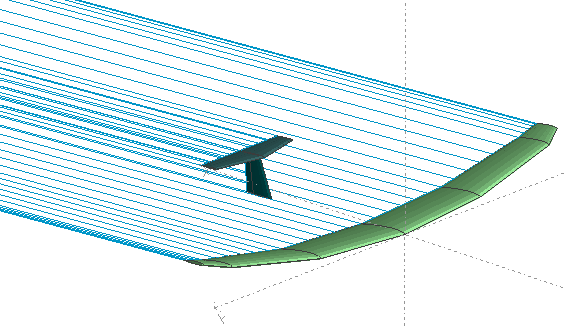
\includegraphics[width=0.8\linewidth]{img-13}\centering 
  \caption{Straight wake}
  \label{fig:straight_wake}
\end{figure}

In a more refined and realistic implementation, the wake is aligned
with the streamlines which trail behind the wing. Since the doublet
distribution on the wing, and the streamlines, in turn depend on the
wake shape, an iteration process is required to reach a converged
state. This is usually referred to as the"wake relaxation process".

The wake relaxation is a difficult process which can easily diverge.
Numerical experimentations in XFLR5 have shown that the wake panels
are highly warped at the wing tips where the wake strongly rolls up on
itself. The convergence requires close control by the user of key
parameters such as number of wake panels, length of wake panels or
time steps. For these reasons, the wake roll-up process has been
disabled.

The wake panels are therefore defined as flat panels which extend
behind the wings trailing edges. Their length is 100 x MAC. At this
distance, the influence of the plane's panels is negligible.

A difficulty arises whenever one of the straight wake panels shed by a
surface such as the wing, goes through another surface such as the
elevator, as illustrated in
Figure~\ref{fig:wake_interference_between_wing_and_elevator}a. This
will lead to unrealistic, non physical results.

In such a situation, it is necessary to modify slightly the geometry
to avoid the interference
Figure~\ref{fig:wake_interference_between_wing_and_elevator}b.

\begin{figure}[htbp]
  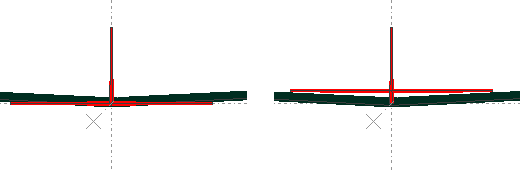
\includegraphics[width=0.8\linewidth]{img-14}\centering 
  \caption{a \& b : Wake Interference between wing and elevator}
  \label{fig:wake_interference_between_wing_and_elevator}
\end{figure}

\subsubsection{Symmetry}
\label{sec:symmetry}

A symmetric calculation reduces the matrix's size by approximately
half (exception is the fin), and reduces the matrix inversion
operations by a factor 4. The code detects automatically whether the
problem is symmetric or not. It is considered to be symmetric in the
following cases :

\begin{itemize}
\item The wing is symmetric in a Wing-only calculation
\item The plane is symmetric without a fin, or with a double fin
\end{itemize}

The problem is asymmetric otherwise :

\begin{itemize}
\item if any of the wings, elevator or fin is asymmetric
\item if the plane has a fin
\end{itemize}

\subsection{Performance analysis}

\subsubsection{Theory - General}

XFoil provides unique insight in the behavior of airfoils, but is a 2D
analysis, hence the results are those of a wing of infinite aspect
ratio and which is defined with a single airfoil. The influence that
the aspect ratio alone may have on the wing's polars, let alone the
sweep or the dihedral, justifies the need for a more sophisticated
wing analysis.

\begin{figure}[htbp]
  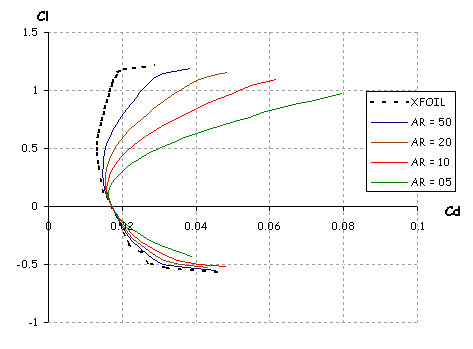
\includegraphics[width=0.8\linewidth]{img-15}\centering 
  \caption{Influence of Aspect Ratio - LLT Calculation NACA 3412 Airfoil - Taper Ratio = 1 - Sweep = $0^\circ$}
  \label{fig:influence_of_aspect_ratio}
\end{figure}

The wing may be computed by either one of three methods, each having
its own advantages, and all having some usage restrictions. \newline
The first is a Lifting Line method, derived from Prandtl's wing
theory. The second is a Vortex Lattice method. The third is a 3D panel
method.\newline
The originality of the implementations is their coupling with XFoil
calculation results to estimate the viscous drag associated with the
wing, although this is done in a different manner depending on the
method.


\subsubsection{Viscous and inviscid calculations}

In VLM and panel methods, an inviscid analysis/polar may be defined,
in which case there is no need to define a polar mesh for the
foils. The viscous characteristics will be set to zero.

The LLT is necessarily viscous.

\subsubsection{Lifting Line Theory (LLT) - Non Linear}

\paragraph{General}

The 'classic' LLT is linear, i.e. the relation $C_l = f(\alpha)$ is
linear, and viscous effects are not taken into account. In the present
application, a non-linear LLT has been implemented based on the NACA
technical note 1269 \cite{Sivells47}.

Quote from Technical Note 1269 :

\begin{quotation}
The hypothesis upon which the theory is based is that a lifting wing
can be replaced by a lifting line and that the incremental vortices
shed along the span trail behind the wing in straight lines in the
direction of the freestream velocity. The strength of these trailing
vortices is proportional to the rate of change of the lift along the
span. The trailing vortices induce a velocity normal to the direction
of the free-stream velocity. The effective angle of attack of each
section of the wing is therefore different from the geometric angle of
attack by the amount of the angle (called the induced angle of attack)
whose tangent is the ratio of the value of the induced velocity to the
value of the freestream velocity.  The effective angle of attack is
thus related to the lift distribution through the induced angle of
attack. In addition, the effective angle of attack is related to the
section lift coefficient according to two-dimensional data for the
airfoil sections incorporated to the wing.  Both relationships must be
simultaneously satisfied in the calculation of the lift distribution
of the wing.

If the section lift curves are linear, these relationships may be
expressed by a single equation which can be solved analytically. In
general however, the section lift curves are not linear, particularly
at high angles of attack, and analytical solutions are not feasible.
The method of calculating the spanwise lift distribution using
non-linear section lift data thus becomes one of making successive
approximations of the lift distribution until one is found that
simultaneously satisfies the aforementioned relationships.
\end{quotation}

The present implementation, the non linear lift behavior is
interpolated on pre-generated meshes of XFoil Type 1 polars and the
non-linearity is solved by an iteration loop :

\begin{figure}[htbp]
  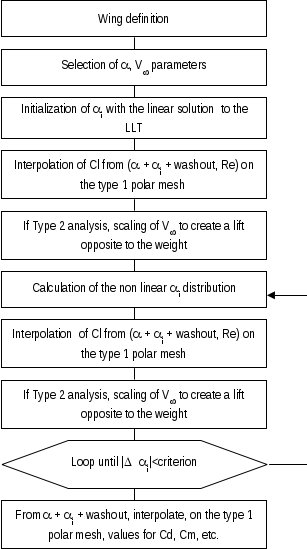
\includegraphics[width=0.5\linewidth]{dia-01}\centering 
\end{figure}

\begin{figure}[htbp]
  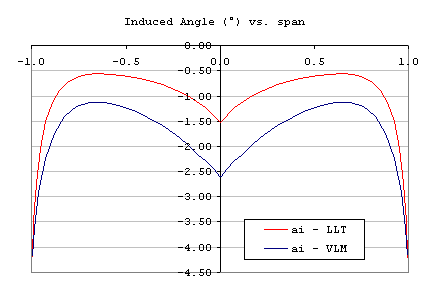
\includegraphics[width=0.8\linewidth]{img-16}\centering 
  \caption{Induced Angle -- Bi-Airfoil NACA3412-NACA1410 -- AR = 14.8 -- TR = 2.0 -- $Alfa = 5^\circ$ - V= 16.7m/s}
  \label{fig:induced_angle}
\end{figure}

\paragraph{Limitations of the LLT}

It is important to note that the lifting line theory has two main
limitations. Quote from Technical Note 1269 \cite{Sivells47} :

\begin{quotation}
The calculations are subject to the limitations of
lifting line theory and should not be expected to give accurate results
for wings of low aspect ratio and large amounts of sweep
\end{quotation}

In addition, the wing's planform is expected to lie
essentially in the X-Y plane, i.e. with low dihedral.

\paragraph{Precautions with the LLT}

As it turns out, the convergence of the non-linear LLT is not a robust
process, and requires careful use of a relaxation factor. This factor
should always be greater than 1. A value of 20 is usually a good
start, and may be increased as necessary for convergence. \newline
Usually wings with low aspect ratio require high relaxation value.

The number of stations across the wing span should be chosen around
20, but may be increased up to 40. Greater numbers do not improve the
precision of the analysis, but tend to seriously hinder the
convergence. The relaxation factor should be increased with higher
numbers of span stations.

\paragraph{2D vs. 3D}

The LLT assumes implicitly that all the surfaces lie essentially in
the X-Y plane.\newline
The only use for the sweep and the dihedral in this implementation of
the LLT is for the calculation of the pitching moment coefficient Cm.
\newline
Sweep and dihedral are not used in the calculation of the lift
distribution.

\paragraph{Viscous and inviscid calculations}

There is no option available to perform a non-viscous LLT calculation.
The reason behind is that the linear theory requires that a zero-lift
angle be defined for each airfoil, and that there is no convenient
manner to define this $\alpha_0$ value which depends on the Reynolds
number.

\paragraph{Lift center of pressure}

Up to v3.11, the position of the lift center at each span location has
been calculated using the usual approximation for thin airfoils, i.e.
: \[X_{CP} = 0.25 - \frac{C_m0}{C_l}\]

From v3.12 onwards, the wing's Center of Pressure's x-position is
calculated by interpolation of the center of pressure's position on
the foil's polar mesh.

For foil polar meshes generated prior to v3.05, the foil's center of
pressure was not stored, hence the formula above is used to calculate
the wing's center of pressure.

\paragraph{Downwash}

The downwash is defined at each span station as
\[V_i = V_\infty sin(\alpha_i)\]

For convenience, it is represented at the wing's trailing edge in 3D
views.

\subsubsection{Vortex Lattice Method (VLM) - Linear }

\paragraph{VLM General principles}

A VLM method has been implemented as an alternative, for the analysis of
those wing geometries which fall outside the limitations of the LLT.

The main differences from the LLT are: 

\begin{itemize}
\item The calculation of the lift distribution, the induced
angles and the induced drag is inviscid and linear i.e. it is
independent of the wing's speed and of the
air's viscous characteristics.
\item The method is applicable to any usual wing geometry,
including those with sweep, low aspect ratio or high dihedral,
including winglets.
\end{itemize}

The principle of a VLM is to model the perturbation generated by the
wing by a sum of vortices distributed over the wing's planform. The
strength of each vortex is calculated to meet the appropriate boundary
conditions (BC), i.e. non penetration conditions on the surface of the
panels.

A comprehensive description of the principles of VLM analysis is well
outside the scope of this document. Only the main features necessary
to a sound use of the code are detailed hereafter.

The resolution of the VLM problem requires the inversion of a square
matrix of the size of the number of panels. This inversion is
performed by Gauss' partial pivot method. The problem's size may be
significantly reduced by considerations of symmetry, detailed in
\S\ref{sec:symmetry}.

\begin{figure}[htbp]
  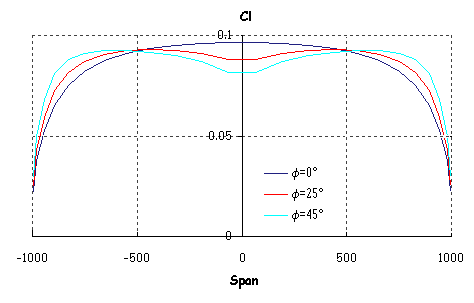
\includegraphics[width=0.8\linewidth]{img-17}\centering 
  \caption{Influence of Sweep for a given CL - AR=10 - TR=1 - Symmetric Airfoil}
  \label{fig:influence_of_sweep}
\end{figure}

\paragraph{Lift force and lift coefficient}

The force acting over each panel is the vector cross product

\[F = \rho V \times \Gamma \]

$\Gamma$ being the vortex strength x its length\\
$\rho$ is the fluid density\\
V is the freestream speed

Which implies that the force is normal to each panel.

The lift coefficient is defined as 

\[C_L = \frac{1}{\rho S V^2} \underset{panels}\sum{F_{wz}}\]

S is the sum of the panels'area, i.e. the planform's area\\
$F_{wz}$ is the projection on the vertical wind axis

This formula is applicable both to a chordwise strip and to the wing's
total surface.

The pitching moments and center of pressure position at each span
location are calculated by summation of the lift force over the
panels.

\paragraph{Limitations of the VLM}

\begin{enumerate}
\item The VLM algorithms first computes the lift coefficient Cl and
the other values which may be calculated by integration of the surface
forces, i.e. the moment coefficients and the center of pressure's
position. The viscous variables (viscous Cd, transitions, etc) are
interpolated from the value of Cl on the previously XFoil-generated
polars. This obviously raises an issue for high and low Cl, where the
Type 1 polar curve may be interpolated either before or after the
stall angle.\newline
VLM results should therefore not be considered around angle of attack
values close to stall angles.
\item In the current formulation, the VLM makes the assumptions of the
small angle of attack. As a main consequence, the trailing vortices
are not aligned with the freestream velocity. This means that the
influence matrix will be independent of the a.o.a.\newline
To explore this limitation, it is possible to experiment a calculation
of the tilted geometry, as explained in
\S\ref{sec:tilted_geometry}. The results tend to show that the
assumption of small angles of attack is acceptable.
\end{enumerate}

\paragraph{VLM alternative method}

In the "classic" VLM method, a horseshoe vortex is positioned at the
panel quarter chord and the non-penetration condition is set at the
three-quarter chord point.

\begin{figure}[htbp]
  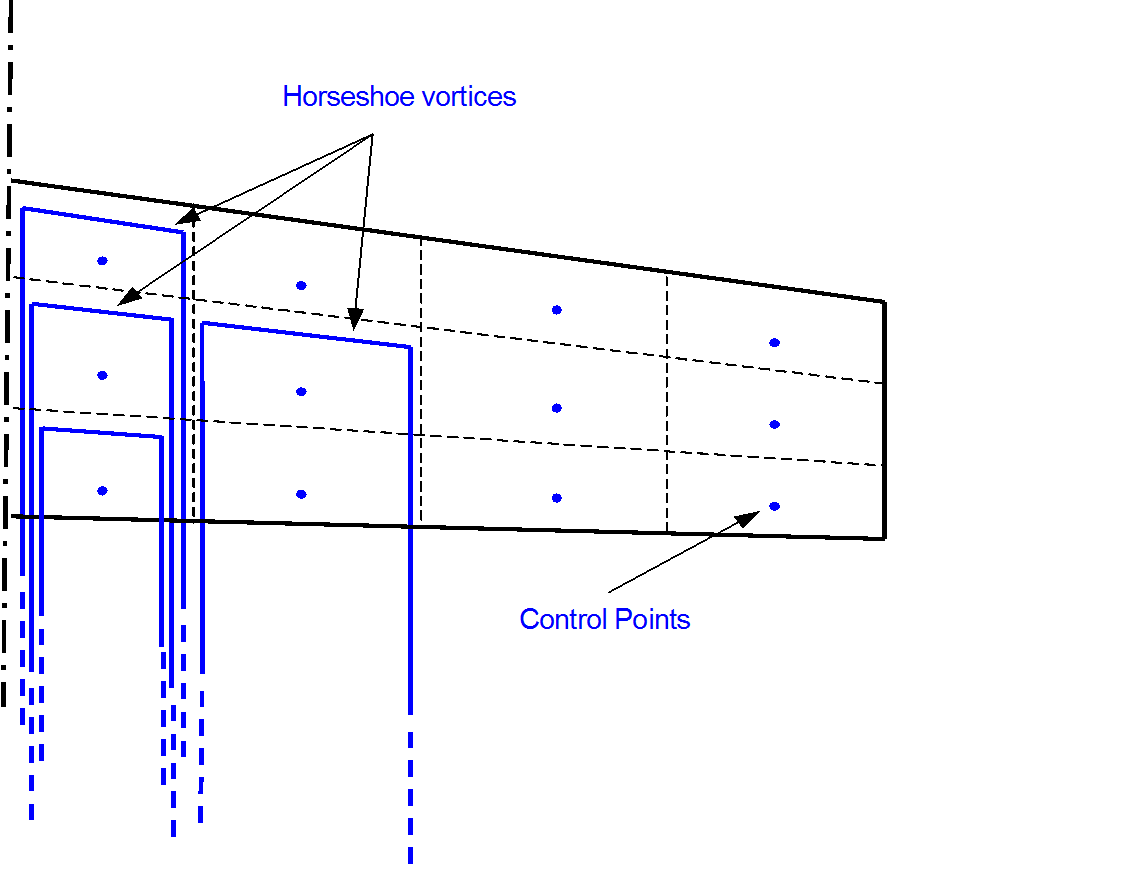
\includegraphics[width=0.8\linewidth]{img-18}\centering 
  \caption{Classic VLM Method}
  \label{fig:classic_vlm_method}
\end{figure}

In the method recommended by Katz and Plotkin \cite{Katz}, only the
trailing vortices extend to infinity.

\begin{figure}[htbp]
  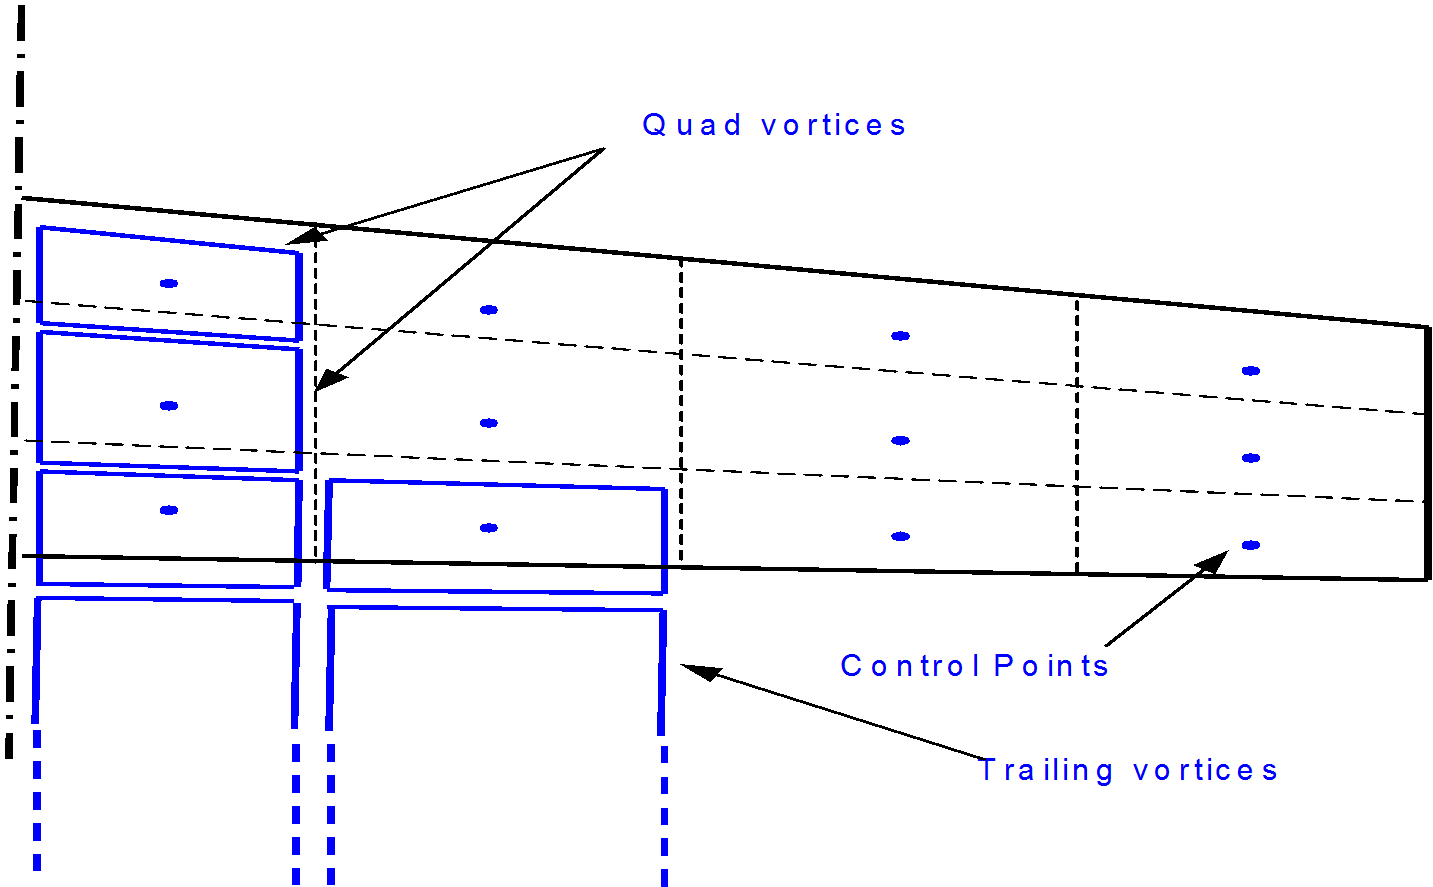
\includegraphics[width=0.8\linewidth]{img-19}\centering 
  \caption{Quad VLM Method}
  \label{fig:quad_vlm_method}
\end{figure}

Since the wake must be force free, the strength of the trailing vortex
is equal to that of the trailing edge quad vortex.

Both methods are implemented for comparison, but give close if not
identical results in most cases.

\paragraph{Panel disposition for VLM}

The resolution of the system and the determination of the vortices'
strengths require a matrix inversion. In some rare cases, this matrix
may turn out to be singular due to a conflicting disposition of panels
and control points on the wing's planform.

The problem arises when a control point is positioned on the line of a
vortex. This will result in a division by zero. In those cases, manual
re-paneling of the wing is sufficient to fix the problem.

\begin{figure}[htbp]
  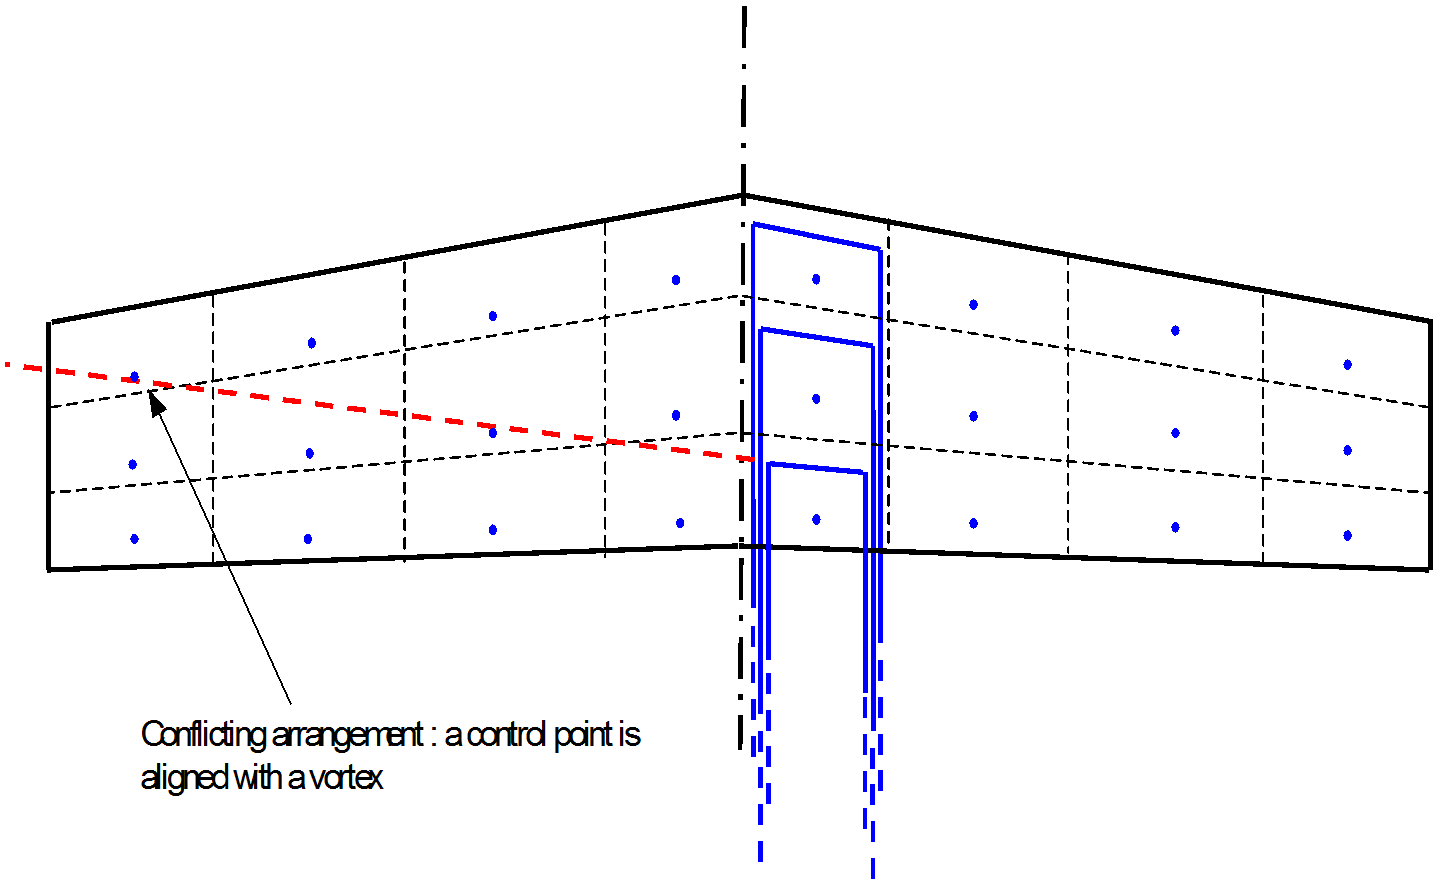
\includegraphics[width=0.8\linewidth]{img-20}\centering 
  \caption{Quad VLM Method}
  \label{fig:quad_vlm_method_2}
\end{figure}

If inversion problems persist despite re-paneling, it will be
necessary to check the consistency of the input data.

\subsubsection{3D Panel Method - Linear}

\paragraph{General Principles}

The 3D panel method has been implemented with the following objectives
:

\begin{itemize}
\item refine the LLT and VLM results by a more sophisticated full 3D
method, taking into account the wings's thickness, whereas the VLM
only considers the mean camber line.
\item provide insight in the Cp distributions over the top and bottom
surfaces of a wing
\item provide a method capable of modeling fuselages
\end{itemize}

The principle of a 3D Panel Method is to model the perturbation
generated by the wing by a sum of doublets and sources distributed
over the wing's top and bottom surfaces. The strength of the doublets
and sources is calculated to meet the appropriate boundary conditions,
which may be of the Dirichlet or Neumann type.

A comprehensive description of the principles of such a method is well
outside the scope of this document. Only the main features necessary
to a sound use of the code are detailed hereafter. The 3D method
implemented in XFLR5 is essentially based on the method in reference
\cite{Maskew}. For those interested, this document provides a
comprehensive review of the theoretical and numerical aspects of the
method.

\paragraph{3D Panel method in XFLR5 v6}

In XFLR5 v6, for a 3D-Panel type, the wing's are modeled differently
depending on whether the analysis is run for a single wing or for a
full plane :

\begin{itemize}
\item for the analysis of a single wing, the wing is modeled as thick
surface, and the full 3D method described in 4 is applied
\item for the analysis of a plane, the fuselage/body is taken into
account, and the wings are modeled as thin surfaces; this is a
restriction due to the impossibility to generate appropriate
connections between wing and body without the help of a 3D-CAD
program.
\end{itemize}

In reference \cite{Maskew}, the authors propose to model the
circulation on the wings using uniform strength doublets, and to place
the Neumann type boundary condition at the collocation point, i.e. the
panel's centroid or center of gravity. The alternative is to use a VLM
method, and to place a vortex at the panel's 1/4 chord, and the BC point
at the panel's 3/4 chord.

Both method have been tested, and the second alternative has proved
more precise and reliable. Hence the 3D-panel method retained for
planes is a mix model of uniform source/doublet for thick bodies, and
horseshoe vortices for thin surfaces.

\paragraph{Problem solving}

The resolution of the panel problem requires the inversion of a square
matrix of the size of the number of panels. This inversion is
performed by LU decomposition.

\paragraph{Wake roll-up}

The wake roll-up process has been implemented and tested. However, it
is not considered to be sufficiently robust to be released at this
time, and has been disabled in v4.00.

\paragraph{Boundary Conditions (BC)}

In a VLM calculation, the BC are necessarily of the Neumann type, i.e.
the velocity's component normal to the surface must be zero.

In a 3D-Panel calculation, the BC may be either of the Neumann or
Dirichlet type. In the latter case the velocity's potential on the
panel's inside surface is zero, so that the total potential inside the
body is equal to the freestream velocity's potential.

After a trial and error process, the recommendation is to use
Dirichlet BC rather than Neumann BC. The latter method is more
sensitive to local geometry changes, and leads to less convincing
results. This is also the choice which is implied in reference
\cite{Maskew}. The type of BC can be modified in the"Advanced
Settings" dialog box.

\paragraph{Validation}

\subparagraph{Infinite Cylinder and Sphere Analysis}

The theoretical values for the Cp coefficients of a body in a uniform
flow are :

\begin{itemize}
\item for a cylinder : $Cp = 1.0$ at the leading and trailing edges, and
$Cp = -3.0$ at the lowest and highest points
\item for a sphere : $Cp = 1.0$ at the leading and trailing edges, and $Cp
= -1.25$ at the lowest and highest points
\end{itemize}

These values are calculated within \% by the 3D panel analysis.

\begin{figure}[htbp]
  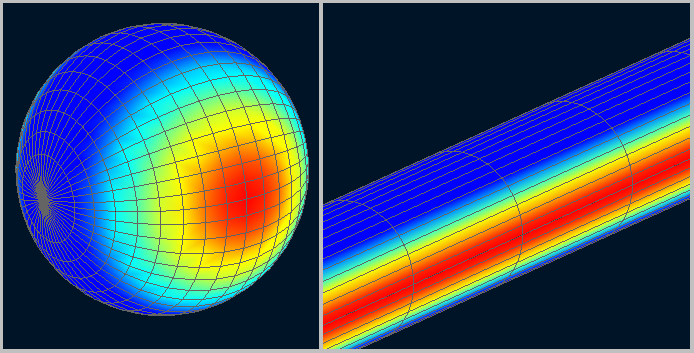
\includegraphics[width=0.8\linewidth]{img-21}\centering 
  \caption{Pressure coefficient Analysis -- Sphere and near infinite cylinder}
  \label{fig:pressure_coeficient_analysis}
\end{figure}

\begin{figure}[htbp]
  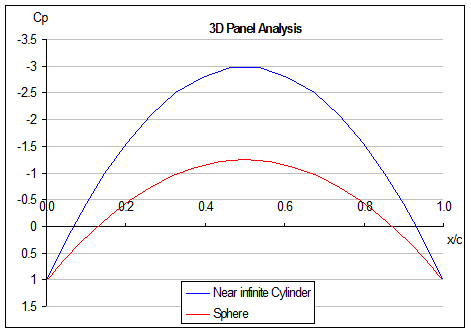
\includegraphics[width=0.8\linewidth]{img-22}\centering 
  \caption{Pressure Coefficient Analysis -- Sphere and near infinite cylinder}
  \label{fig:pressure_coeficient_analysis_2}
\end{figure}

\subparagraph{Wing Analysis}

The Cp distributions calculated by 3D panel analysis for a near
infinite wing, and by 2D panel analysis with XFoil are plotted in
Figure~\ref{fig:pressure_coeficient_analysis_naca2412} and in
Figure~\ref{fig:pressure_coeficient_analysis_naca_64A410}. There is
general concordance for inviscid results.

\begin{figure}[htbp]
  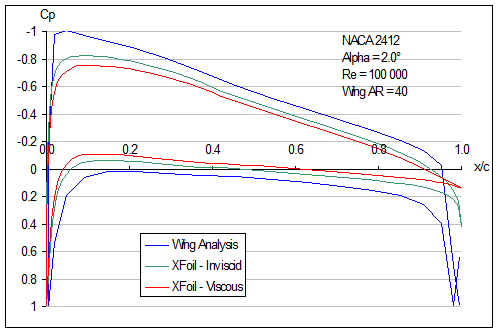
\includegraphics[width=0.8\linewidth]{img-23}\centering 
  \caption{Pressure Coefficient Analysis -- NACA2412}
  \label{fig:pressure_coeficient_analysis_naca2412}
\end{figure}

\begin{figure}[htbp]
  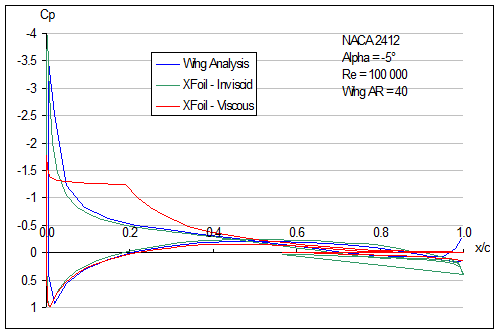
\includegraphics[width=0.8\linewidth]{img-24}\centering 
  \caption{Pressure Coefficient Analysis -- NACA64A410}
  \label{fig:pressure_coeficient_analysis_naca_64A410}
\end{figure}


\subsubsection{Analysis considerations}

\paragraph{General Limitations}

As a general rule, LLT and VLM are adapted to configurations of thin
lifting surfaces, operating at small angles of attack.

The most questionable assumption of the wing design algorithm is
probably the use of XFoil transition results to wings with finite
aspect ratio. The 2D simulation proposed by XFoil corresponds to
infinite wings, where a laminar bubble extends indefinitely along the
span. Some authors suggest that on span-limited wings, such bubbles
will appear only on a fraction of the planform. However, theories for
3D transitions are still in development and to the author's knowledge,
not giving total satisfaction yet.

The method which consists in interpolating XFoil generated results is
clearly an approximation with no real theoretical or experimental
background, but should be a reasonable approximation for wings with
moderate to high aspect ratio.

The viscous characteristics will be less and less representative as
the wing geometries differ from the ideal 2D Xfoil infinite
wing. Hence those results for non planar geometries, low aspect ratio
or high sweep should be considered with caution.

\paragraph{Selection of an Analysis Method}

The LLT method should always be preferred if the wing's geometry is
consistent with the limitations of the theory. LLT provides better
insight into the viscous drag, gives a better estimation of the
behavior around stall conditions at high angles of attack, and is
better supported by theoretical published work.

The 3D panel method should be selected if there is interest in the Cp
distribution on top and bottom surfaces, or if the body's influence
should be taken into account.

VLM analysis is preferable for all other cases.

The comparison of the Cp distribution at two span positions for
different method of analysis is given in
Figure~\ref{fig:cp_comparison_for_different_analysis_methods} and
Figure~\ref{fig:cp_comparison_for_different_analysis_methods_2}.

\begin{figure}[htbp]
  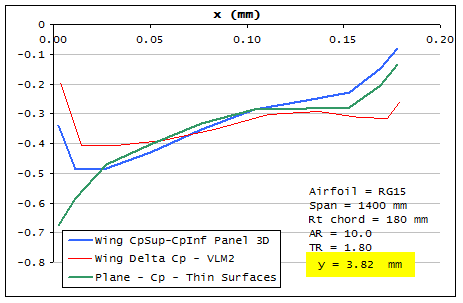
\includegraphics[width=0.8\linewidth]{img-25}\centering 
  \caption{Cp comparison for different analysis methods}
  \label{fig:cp_comparison_for_different_analysis_methods}
\end{figure}

\begin{figure}[htbp]
  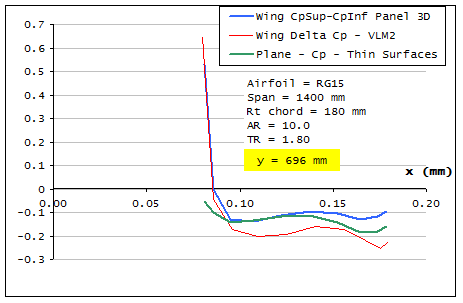
\includegraphics[width=0.8\linewidth]{img-26}\centering 
  \caption{Cp comparison for different analysis methods}
  \label{fig:cp_comparison_for_different_analysis_methods_2}
\end{figure}

\paragraph{Core radius}

In VLM analysis, the velocity vector induced by a vortex is singular
on the vortex line.

In a 3D panel method, the velocity vector is singular in the alignment
of the panel sides.

This can create numerical errors in the analysis and in the
calculations of the streamlines.

It is therefore highly recommended to set a minimal core radius, which
can typically be of the order of magnitude of 1/1000 of the min mesh
panel size, e.g. $Core radius = 10^{-6}m$. This is the value set by
default, and it can be modified in the advanced settings.

The velocity at a point located on the vortex line, or in the
alignement of a panel side, is zero.

\paragraph{Sideslip}

The simulation of sideslip has been introduced in XFLR5 v4.09.

The order in which a.o.a. and sideslip are applied has its importance.
In XFLR5, sideslip is modeled by rotating the model about the z-axis,
with a freestream velocity vector remaining in the x-z plane. The
resulting geometry is analyzed using the conventional VLM and panel
methods. The advantage of this method is that the trailing vortices
are in the vertical plane which contains the velocity vector, i.e. are
aligned with the x-axis of the stability frame.

\begin{figure}[htbp]
  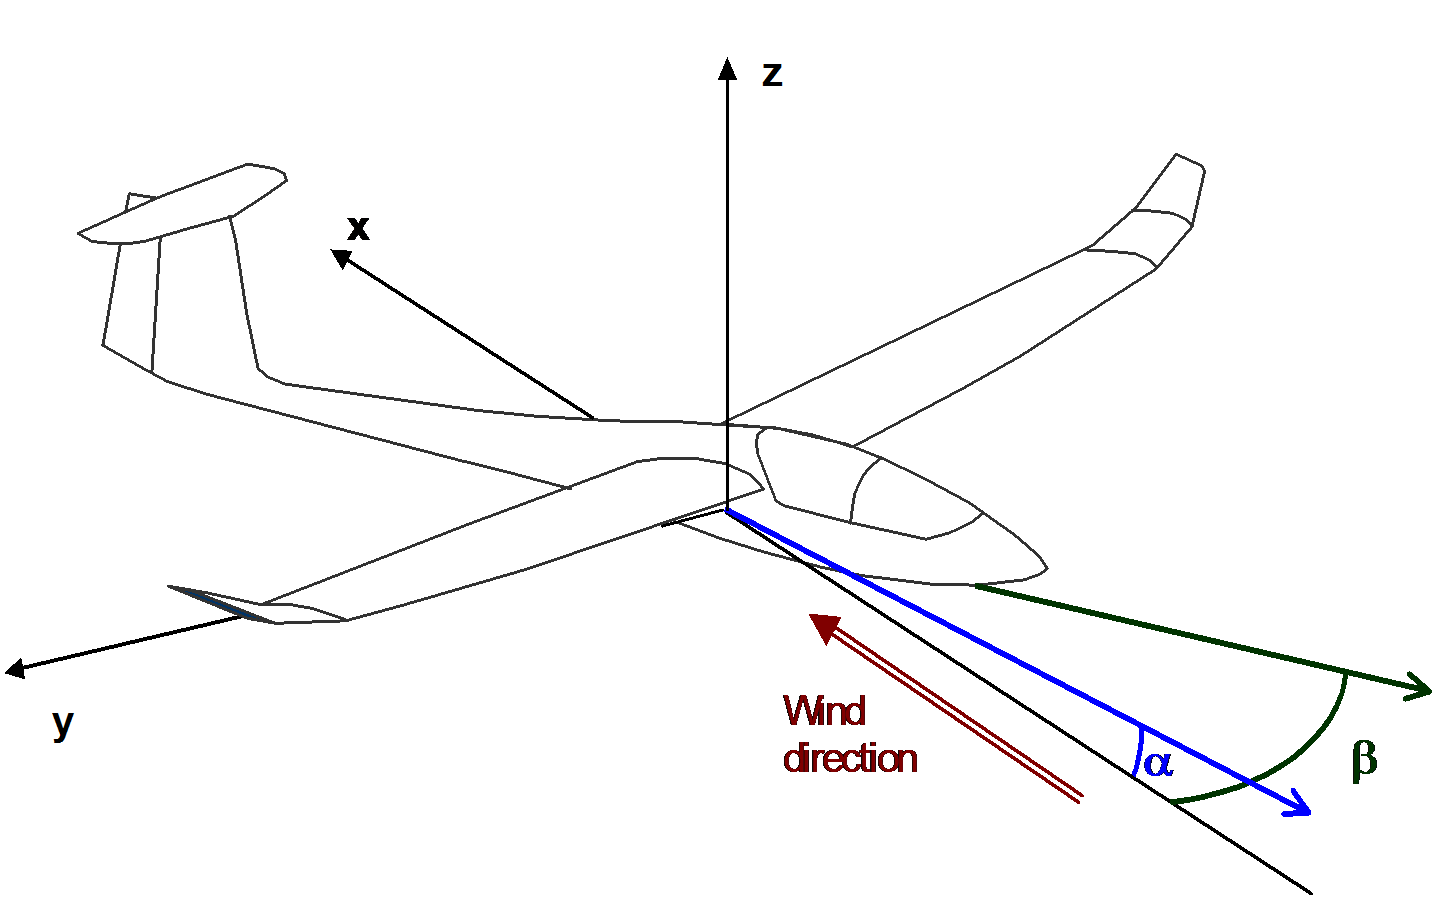
\includegraphics[width=0.8\linewidth]{img-27}\centering 
  \caption{Definition of sideslip}
  \label{fig:definition_of_sideslip}
\end{figure}

\paragraph{Trefftz Plane, far field and near field analysis}

The lift and induced drag may be calculated by near field or by far
field methods. The theoretical aspects are too vast to be detailed
here, but in essence the near field method consists in an integration
of pressure forces on the panels, whereas the far field method is
based on the balance of the momentum on a control surface far
downstream of the body, i.e. the Trefftz plane.

It is generally reported that the drag and lift results from near
field analysis are significantly higher and less representative than
those resulting from a calculation in the Trefftz plane. This issue is
not specific to the present implementation, but is reported for almost
all VLM and panel codes. The implementation in the present code for
the calculation of lift and drag is therefore the far field method.

On the other hand, far field analysis does not provide information on
the pressure distribution over the strip, and no information on the
pitching moment with reference to the chord's quarter point. All the
moments and the position of the center of pressure are therefore
calculated by summation on the panels.

In the current implementation of the 3Dpanel method, it is considered
that only the wings shed a wake, and that the body does not.

\paragraph{Linear and non-linear behavior}

Traditional VLM and Panel analysis do not account for viscous effects.
For model aircraft operating at a few m/s however, the viscous drag is
not negligible compared to the induced drag, and must therefore be
estimated by an alternative mean.

In the present application, the viscous drag is estimated by
interpolation of XFoil pre-generated polars, by the Cl value resulting
from the linear 3D analysis. This assumes implicitly that the foil's
behavior on a finite wing is not very different than on an "infinite
XFoil wing". There is no real background, neither theoretical nor
experimental, to support this approach, so it should be used with
caution.

As is generally the case when transposing 2D results to 3D analysis,
the estimation of viscous drag is probably too low and may lead to
arguably optimistic results.

Because the VLM is linear, it does not, among other things, account
properly for stall at high angles of attack, unlike, potentially, the
LLT.

\begin{figure}[htbp]
  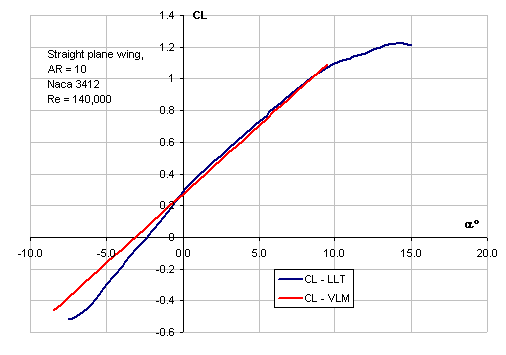
\includegraphics[width=0.8\linewidth]{img-28}\centering 
  \caption{Linear and Non-Linear modeling}
  \label{fig:linear_and_non_linear_modeling}
\end{figure}


\paragraph{Non-Linear Implementation}

\begin{figure}[htbp]
  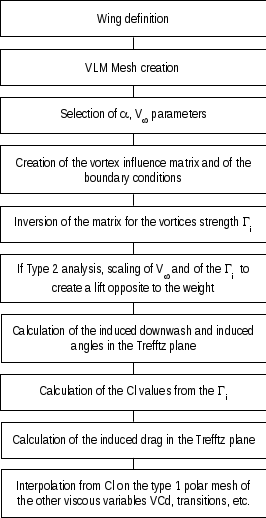
\includegraphics[width=0.5\linewidth]{dia-02}\centering 
\end{figure}

\paragraph{Tilted Geometry -- VLM and 3D Panel Analysis}
\label{sec:tilted_geometry}

The baseline VLM method uses small angle approximation for the wake's
definition. Within this assumption, the wake is aligned with the body
axes :

\begin{itemize}
\item For VLM, the trailing legs of the horseshoe vortices are
parallel to the body's x-axis (Figure~\ref{fig:normal_and_tilted_geometry_configurations}a).
\item For 3D Panel analysis, the trailing wake panels are in
the x-y plane
\end{itemize}

The advantage of this approximation is its simplicity : only one
influence matrix is required for all angles of attack, and the matrix
inversion can be performed for all alphas simultaneously.\newline
The disadvantage is that the horseshoe vortices or the wake panels are
not aligned with the freestream velocity.

\begin{figure}[htbp]
  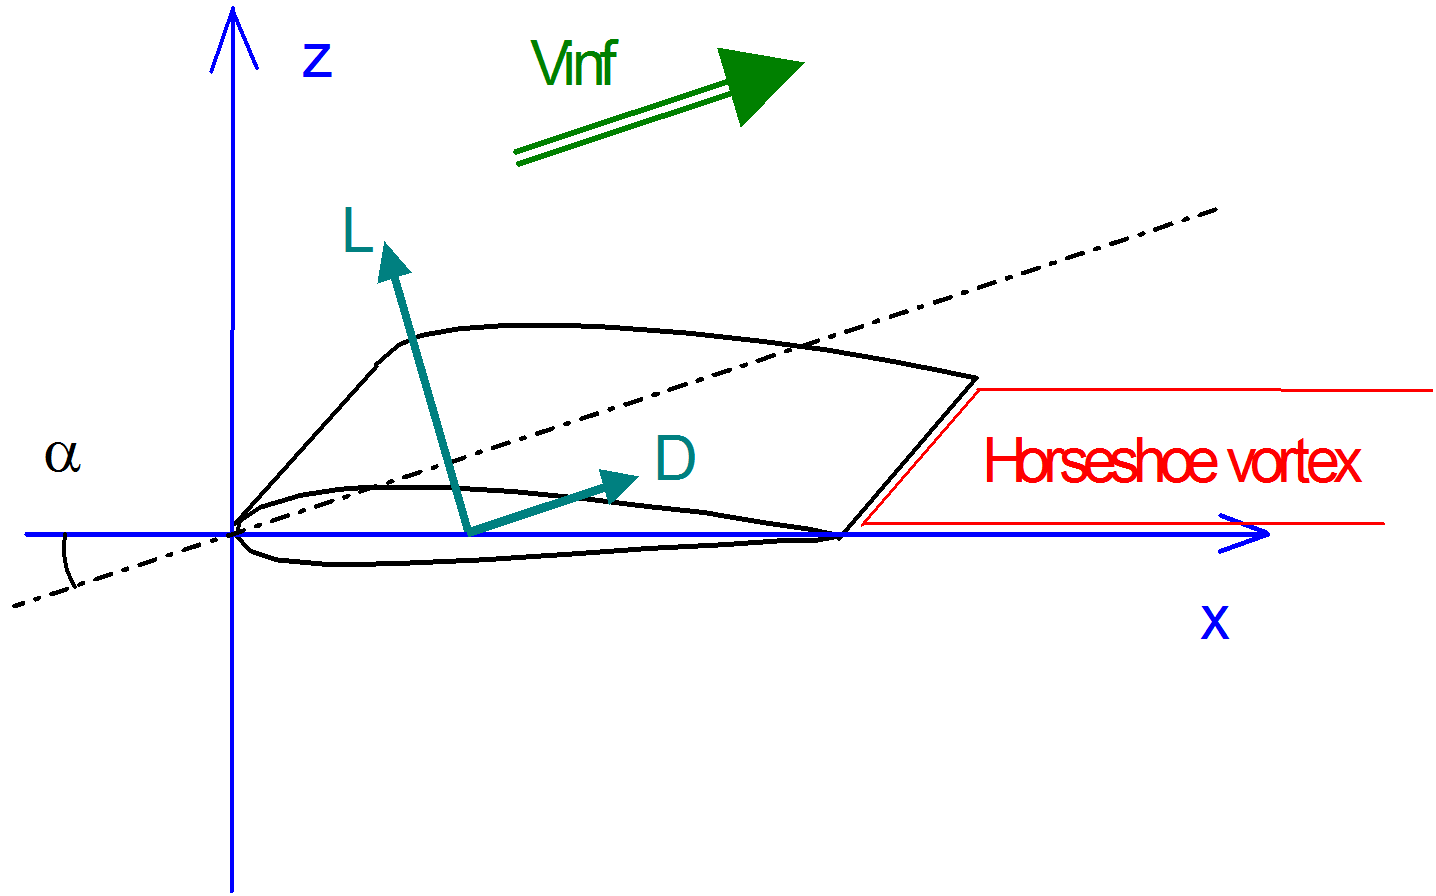
\includegraphics[width=0.8\linewidth]{img-29}\centering\\
  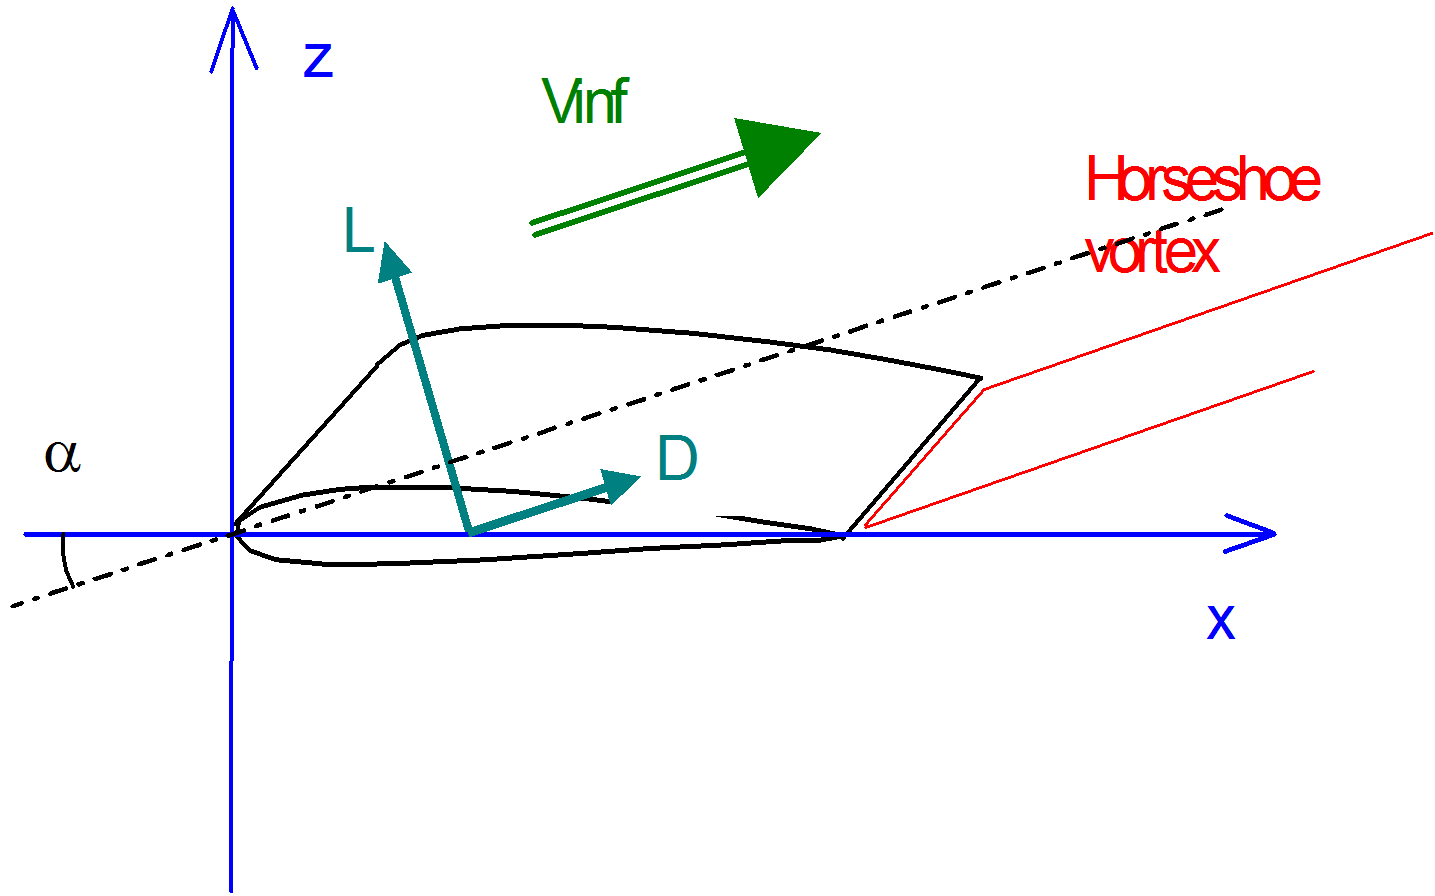
\includegraphics[width=0.8\linewidth]{img-30}\centering\\
  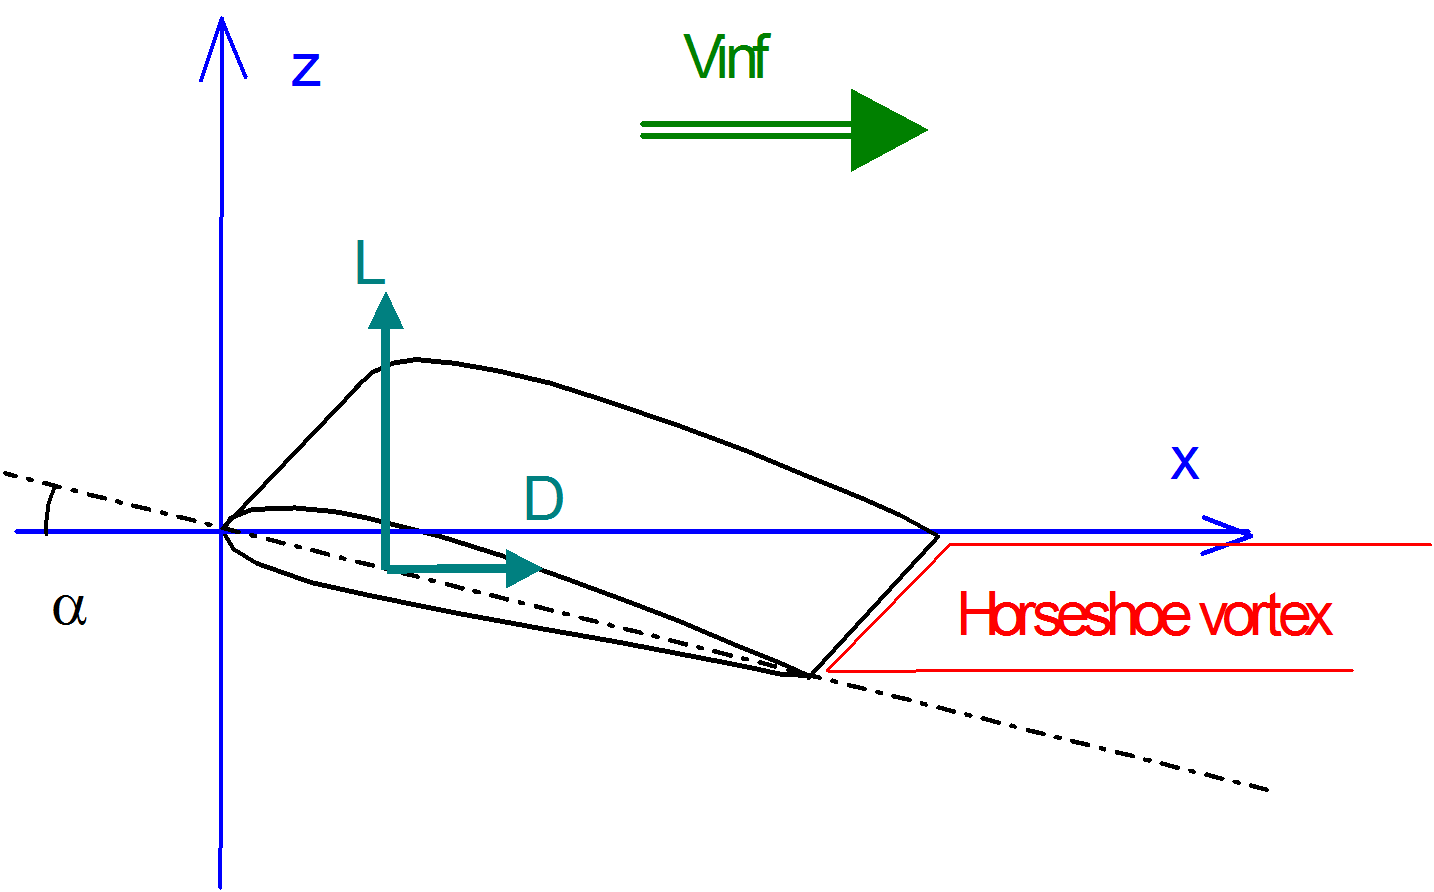
\includegraphics[width=0.8\linewidth]{img-31}\centering
  \caption{Normal and Tilted geometry configurations}
  \label{fig:normal_and_tilted_geometry_configurations}
\end{figure}


A more representative approach is to align the wake with the wind axes
(Figure~\ref{fig:normal_and_tilted_geometry_configurations}b). Equivalently,
the problem can be set in the wind axes and the body's geometry can be
tilted by the angle of attack
(Figure~\ref{fig:normal_and_tilted_geometry_configurations}c), which
is a direct transposition of the physics of the problem.  Both methods
are equivalent, but the latter can be implemented more simply, hence
has been chosen for XFLR5. It is selected by checking the "Tilt
Geometry" checkbox in the Analysis Dialog Box.

The inconvenience with this approach is that a new matrix must be set
up and inverted for each angle of attack, leading to longer
computation times.

The coefficients Cl and Cd are almost identical for both methods,
which means the small angles approximation is applicable from the
performance analysis point of view. The moment coefficients may be
slightly different.

\paragraph{Wake roll-up -- VLM and 3D Panel Analysis}

\underline{Note} : Because it is sensitive and difficult to use, the wake roll-up
process has been disabled. The following explanation is provided for
information only.

\subparagraph{General considerations}

In their base formulation, both the VLM and the Panel methods make the
assumption of a flat wake, which is an approximation. The wake tends to
roll up on itself, which can be illustrated for instance by the two
vortices at the tip of each wing.

A wake model more refined than the simple straight line or flat panel
can be of interest for two reasons :

\begin{itemize}
\item Although the wake carries no load and therefore has no
influence on the lift coefficient, its shape affects the induced drag
value and derived coefficients
\item A flat wake is inappropriate for plane configurations
with and elevator, since the downwash created by the main wing
influences the flow field around the elevator.
\end{itemize}

The shape of the wake is determined by the flowfield behind the wing,
but in turn, the flow field is dependent on the wake shape. Therefore,
the shape the wake takes in a constant state situation can be deduced
by an iterative process, in which the wake geometry is updated
("relaxed") after each computation loop.

\subparagraph{Wake mesh}

The panels formulation implemented in XFLR5 is
of the constant, flat panel type. Special care must therefore be taken
in the choice for the wake
panel's size, to avoid excessive twisting. The panel
size is controlled by three parameters :

\begin{itemize}
\item The wake's total length
\item The streamwise size for the first wake panel's length
\item The ratio, or progression factor, between two adjacent panels in the
streamwise direction
\end{itemize}

As a general indicaction, it is advisable to set those parameters so
that the first panel's size is approximately the same
as that of the wing's trailing edge panel.

\subparagraph{Roll-up process}

Ideally, the lift and drag coefficients tend towards limit values.
However, if no special precautions are taken, numerical experiments
show that the wake tends to roll up indefinitely on itself. This leads
to highly twisted panels and to numerical divergence.

Since the roll-up is not a robust process, the iteration loop is
limited both by the number of iterations and by a precision criterion.

\begin{figure}[htbp]
  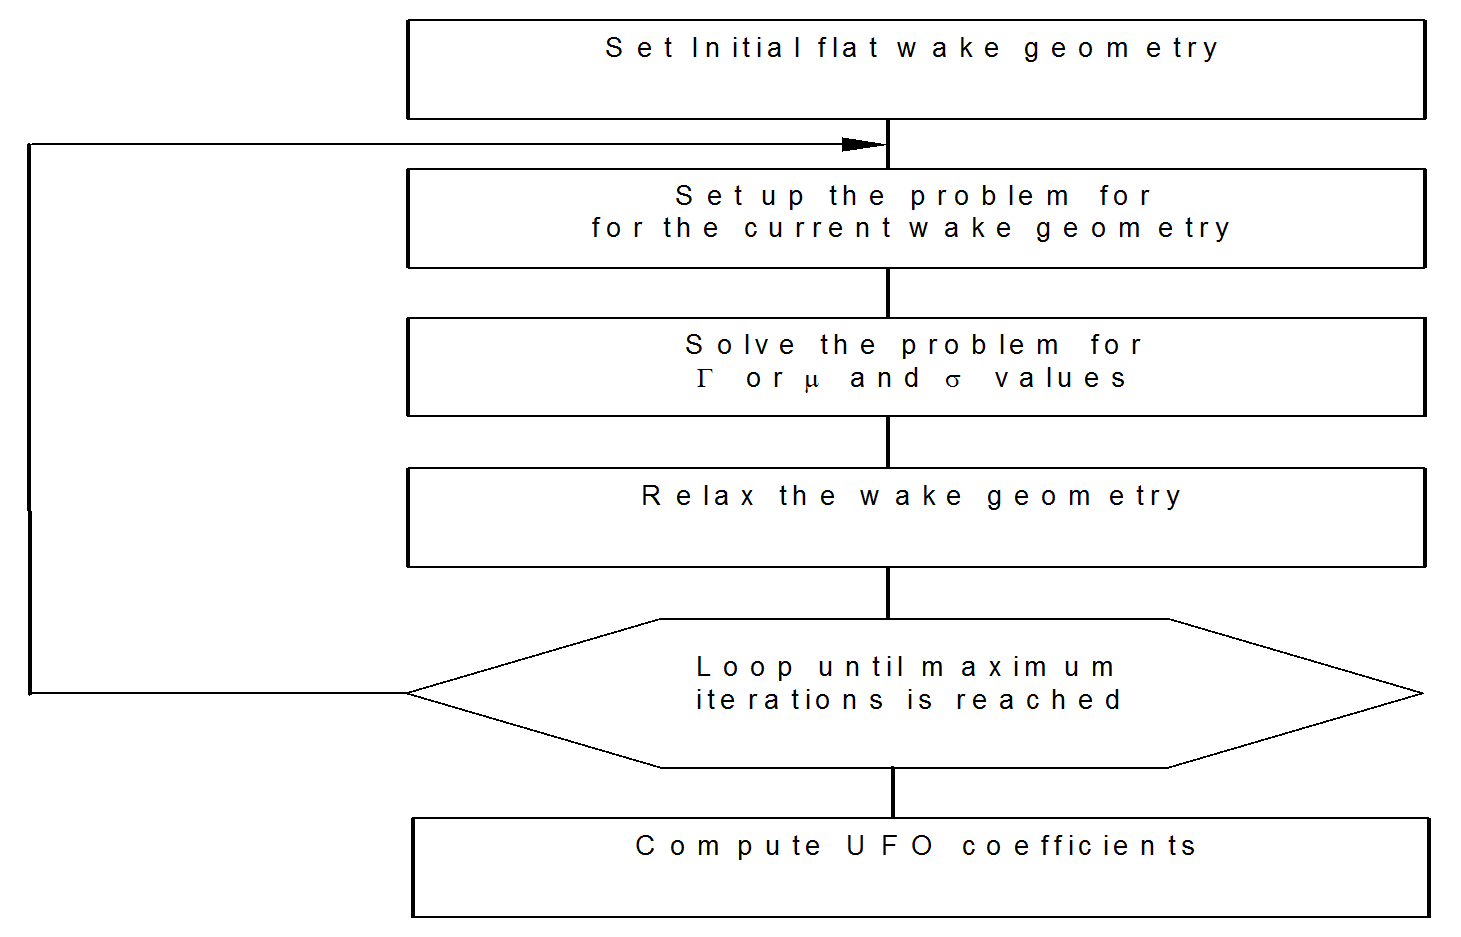
\includegraphics[width=0.8\linewidth]{img-32}\centering 
  \caption{Wake roll-up iteration process}
  \label{fig:wake_roll_up_iteration_process}
\end{figure}

Reference \cite{Werner} provides a comprehensive description of the issues related
to wake roll-up.

\subsubsection{Moments}
\label{sec:moments}

All moment calculations in LLT are strictly in accordance with the
formula of NACA TN1269.

In V4.00, the definition of the moments has been modified to clarify
some ambiguities that existed up to v3.21.

From V4.00 onwards, the geometric pitching, rolling and yawing moments
are calculated by integration of forces on the panels. For VLM this is
done at the vortex middle position, for 3D Panel analysis, the force is
applied at the panel's center.

The geometric moments are therefore the total moments applied to the
wing or plane.

For analysis purposes, it may be interesting to break down those moments
in separate parts, or to isolate one specific contribution to the total
moment.

\underline{Strip Moment Coefficients}

These moments are calculated for each span position on the wing and are
accessible in the Operating Point graphs.

\begin{table}[htbp]\scriptsize
  \centering
  \begin{tabular}{|*{4}{m{0.03\linewidth}|}*{3}{m{0.19\linewidth}|}}
    \hline
    \multicolumn{2}{|c|}{Moment} &
    Sign &
    Ref.\newline Len. &
    Nature &
    LLT &
    VLM \& 3D Panel\\
    \hline
    \multirow{2}{0.03\linewidth}{\begin{sideways}Pitching\end{sideways}} & 
    \begin{sideways}Airfoil $C_m$~Airfoil\end{sideways} & 
    \multirow{2}{0.03\linewidth}{\begin{sideways}positive nose~up\end{sideways}} & 
    \multirow{2}{0.03\linewidth}{\begin{sideways}M.A.C : $M=q.S.mac.C_m$\end{sideways}} & 
    Moment of the lift forces around the 1/4 chord point&
    The value for the pitching moment is interpolated on the foil's polar
    mesh. It takes into account viscous effects&
    Sum of the moments created by pressure forces on the strip's panels
    The viscous part is ignored \\
    \cline{2-2} \cline{5-7}
    &
    \begin{sideways}$C_m$\end{sideways} &
    &
    &
    Moment of the pressure and viscous forces with respect to XCmRef&
    Integration over the wing's lifting line of the strips self pitching
    moment, and of the strip lift force Both sweep and dihedral are taken
    into account&
    Sum on all the panels of the moments of pressure forces + pitching
    moment of viscous drag forces \\
    \hline
  \end{tabular}
  \caption{Strip Moment Coefficients}
  \label{tab:strip_moment_coefficients}
\end{table}

\underline{Wing moment coefficients}

\begin{table}[htbp]\scriptsize
  \centering
  \begin{tabular}{|*{4}{m{0.03\linewidth}|}*{3}{m{0.19\linewidth}|}}
    \hline
    \multicolumn{2}{|c|}{Moment} &
    Sign &
    Ref.\newline Len. &
    Nature &
    LLT &
    VLM \& 3D Panel\\
    \hline % 8<---------------------
    \multirow{3}{0.03\linewidth}{\begin{sideways}Pitching\end{sideways}} & 
    \begin{sideways}Geom (global) $GCm$~Airfoil\end{sideways} & 
    \multirow{3}{0.03\linewidth}{\begin{sideways}positive nose~up\end{sideways}} & 
    \multirow{3}{0.03\linewidth}{\begin{sideways}M.A.C : $M=q.S.mac.C_m$\end{sideways}} & 
    Moment of the pressure forces with respect to XCmRef&
    Integration of the moment over the wing's lifting line.  Both
    sweep and dihedral are taken into account&
    Sum on all the panels of the moments of pressure forces \\
    \cline{2-2} \cline{5-7}
    &
    \begin{sideways}Viscous (global) $VCm$\end{sideways} &
    &
    &
    Moment of the viscous airfoil drag forces with respect to XCmRef&
    \multicolumn{2}{|c|}{Integration of the moment over the wing's
    lifting line.} \\
    \cline{2-2} \cline{5-7}
    &
    \begin{sideways}Airfoil (at local span pos.)\end{sideways} &
    &
    &
    Moment of the lift forces around 1/4 chord point&
    Cm interpolated on polar 1 mesh&
    Sum of the moments created by pressure forces on the strip's panels \\
    \hline % 8<---------------------
    \begin{sideways}Rolling\end{sideways} & 
    \begin{sideways}Geom (global) $GRm$\end{sideways} & 
    \begin{sideways}positive with the starboard wing down\end{sideways} &
    \begin{sideways}Span : $R=q.S.b.C_r$\end{sideways} & 
    Moment of the pressure forces with respect to XCmRef&
    Integration of the lift's moment over the wing's lifting line.
    Dihedral is not taken into account&
    Sum on all the panels of the moments of pressure forces \\
    \hline % 8<---------------------
    \multirow{3}{0.03\linewidth}{\begin{sideways}Yawing\end{sideways}} & 
    \begin{sideways}Geom (global) $GYm$\end{sideways} & 
    \multirow{3}{0.03\linewidth}{\begin{sideways}positive with the nose to starboard\end{sideways}} & 
    \multirow{3}{0.03\linewidth}{\begin{sideways}Span : $N=q.S.b.C_n$\end{sideways}} & 
    Moment of the pressure forces with respect to XCmRef&
    N/A&
    Sum on all the panels of the moments of pressure forces \\
    \cline{2-2} \cline{5-7}
    &
    \begin{sideways}Profile (global) $VYm$\end{sideways} &
    &
    &
    Moment of the viscous airfoil drag forces with respect to the plane y=0&
    \multicolumn{2}{|c|}{Integration of the moment over the wing's
    lifting line} \\
    \cline{2-2} \cline{5-7}
    &
    \begin{sideways}Induced (global) $IYm$\end{sideways} &
    &
    &
    Moment of the induced tangential forces with respect to the plane y=0&
    \multicolumn{2}{|c|}{Integration of the moment over the wing's
    lifting line} \\
    \hline % 8<---------------------
  \end{tabular}
  \caption{Wing moment coefficients}
  \label{tab:wing_moment_coefficients}
\end{table}

\subsubsection{Neutral point, Center of pressure, Static Margin}

XFLR5 up to v3.12 has provided a measure of the quantity \[SM =
\frac{(X_{CP} - X_{CG})}{MAC}\] incorrectly labeled "Static Margin",
where

\begin{itemize}
\item $X_{CP}$ is the centre of pressure's streamwise position
\item $X_{CG}$ is the centre of gravity's streamwise position
\end{itemize}

The conventional static margin of a wing or a plane may be determined
by an iterative process. It is the CG position (or moment reference
position XCmRef) for which \[\frac{dCm}{d\alpha}=0\] This is
illustrated in the Figure~\ref{fig:wing_neutral_point} where the
neutral point is approximately 67 mm from the leading edge.

\begin{figure}[htbp]
  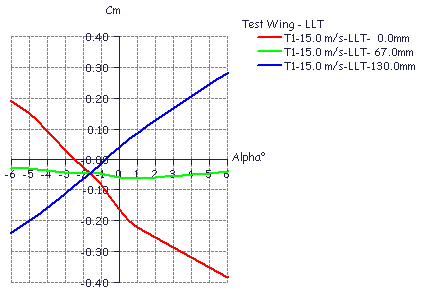
\includegraphics[width=0.8\linewidth]{img-33}\centering 
  \caption{Wing Neutral Point}
  \label{fig:wing_neutral_point}
\end{figure}

Illustration of the way to use XFLR5 to position the CG of a model
sailplane are given in \cite{DeperroisStab} and \cite{DeperroisNotions}.

\subsubsection{Efficiency factor}

The efficiency factor, referred to also as Oswald's factor, is a
measure of the deviations of the wing's induced drag from that of an
optimal elliptic loading, and is defined
as \[e=\frac{CL^2}{\pi.AR.ICd}\] where

\begin{itemize}
\item CL is the lift coefficient
\item ICd is the induced drag coefficient
\item AR is the wing's Aspect Ratio
\end{itemize}

The efficiency factor, also named Oswald's factor, should always be
smaller than 1. It may happen however that this factor becomes greater
than 1 for numerical reasons in LLT, VLM and 3D Panel calculations.

In LLT, this may be corrected by increasing the precision required for
convergence, for instance with the following parameters :

\begin{itemize}
\item Number of stations = 40
\item Relaxation factor = 40
\item convergence criterion = 0.001
\item Max Number of iterations = 300
\end{itemize}

In VLM and 3D Panels, a refinement of the panel density in the
streamwise direction is required to reduce the efficiency factor to
values less than 1.

\subsubsection{Wing Operating Points and Wing Polars}

The presentation of results is the same as for foil analysis,
i.e. each converged analysis generates an operating point and adds
results to a polar object. The definition and selection of an
Analysis/Polar object is necessary to perform a calculation.

Any number of Operating Points may be stored in the runtime database,
the only limitation being computer memory. Wing and plane operating
points will use significant memory resources.

Type 1 and Type 4 polars are unchanged from foil analysis.

A type 2 polar corresponds to a plane with a given weight operating at
constant lift.

For a given angle of attack, the plane's velocity is calculated to
create a lift force opposite to the weight of the airplane
: \[V=\sqrt{\frac{2mg}{\rho SC_l}}\] The angle of descent
is \[\gamma=arctan(\frac{C_d}{C_l})\] and the horizontal and vertical
speeds are respectively \[V_x=V_\infty cos(\gamma)\]
\[V_z=V_\infty sin(\gamma)\]

\begin{figure}[htbp]
  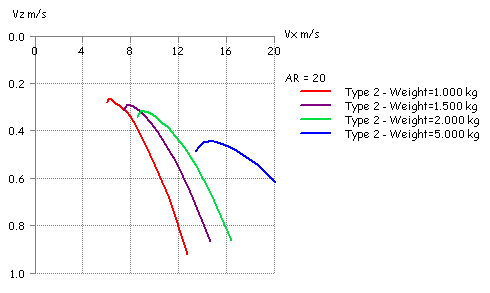
\includegraphics[width=0.8\linewidth]{img-34}\centering 
  \caption{Speed polars based on Type 2 analysis}
  \label{fig:speed_polars_based_on_type_2_analysis}
\end{figure}

Convergence for type 2 polars requires that the apparent angle of
attack be greater than the zero-lift angle. Otherwise, no speed
whatsoever may generate a positive lift...

\subsubsection{Control analysis -- Polar \foreignlanguage{english}{Type 5 and Type 6}}

The Type 5 and Type 6 control polars have been disabled in XFLR5 v6 and
are replaced by the Type 7 stability polars.

\subsubsection{Interpolation of the XFoil-generated Polar Mesh}

The code does not recalculate with XFoil each operating point at every
wing station and at each iteration: 

\begin{itemize}
\item this would require lengthy -and unnecessary- calculations
\item XFoil's convergence is too uncertain
\end{itemize}

Instead, the operating point is interpolated from a pre-generated set
of Type 1 polars.

The wing calculation requires that a set of \textbf{Type 1} foil
polars be previously loaded or generated for each of the wing's
foils.\newline

\begin{figure}[htbp]
  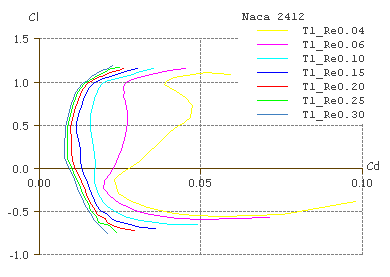
\includegraphics[width=0.8\linewidth]{img-35}\centering 
  \caption{Polar mesh ranging from Re = 40,000 to Re = 300,000}
  \label{fig:polar_mesh_ranging_from}
\end{figure}

The set of polars should cover the whole flight envelope of each point
of the wing, with regard to both Reynolds numbers and to the apparent
angle of attack.

If any point of the wing planform operates outside the available polar
mesh, a warning message is issued in the log file. This happens for
instance in the case of short tip chords of elliptic wings. In such a
case, the "closest point" of the mesh will be used, and the
operating point may be generated and added to the current polar, if so
chosen by the user.

For the interpolation process, the code uses indifferently all
available type 1 polars related to the selected foil. The user must
therefore be careful to provide only a homogeneous and consistent set
of polars.

The interpolation process of a variable X (X being Cl, Cd, Cm,
Transition points etc.) from $[\alpha = aoa + \alpha_i + washout, Re]$
at a geometrical point P between the foils 1 and 2 is:

\begin{enumerate}
\item For the first foil, find polars 1 and 2 such that
$Re_1 <  Re < Re_2$;\newline
if neither polar 1 nor 2 can be found, return on error\newline
if Re is less than all the polars' Reynolds numbers, use the polar of
smallest Re\newline
if Re is greater than that of any polars' number, use the polar of
greatest Re
\item Interpolate each polar with $\alpha$ to get $X_{11}$ and
$X_{12}$\newline
if either polar is not defined up to $\alpha$, use the smallest or
greatest angle available, and issue a warning\newline
if only one polar is available, interpolate only that polar, and issue
a warning
\item Interpolate $X_1$ between $X_{11}$ and $X_{12}$, pro-rata of Re
between $Re_1$ and $Re_2$
\item Do the same for the second foil to get $X_2$
\item Interpolate X between $X_1$ and $X_2$, pro-rata of the position
of the point between the two foils
\end{enumerate}


\subsubsection{Streamlines}

The streamlines are calculated from the vortices, or doublet and
source, strengths each time an operating point is selected.

The calculation is incremental, in the x streamwise direction.

The streamline are initiated at the mesh panels leading edge or
trailing edge, with a user defined offset in the x and z directions.

The "Initial Length" is the first x-increment for the calculation of
the streamline.

The "Progression Factor" determines the length of step n+1 vs. step
n.

Caution note : The velocity vector is singular at the panel edges in
3D-Panel analysis, and on the panel's vortex trailing line in VLM
analysis. This may cause numerical instabilities, in cases for
instance when the streamlines are requested to initiate exactly at the
panels leading or trailing edge, or at the panel corners. A minor x or
z offset is necessary to prevent the instability. The use of a core
radius, which can be defined in the advanced settings, is another
possibility.

\subsubsection{Comparison to experimental results}

The code has been tested against experimental results and against
other software, with consistent results.\newline
Also, the VLM, 3D Panel and LLT algorithms in their XFLR5 implementation
are totally independent, but give close results in the linear part of
the Cl vs. $\alpha$ plots.

\begin{figure}[htbp]
  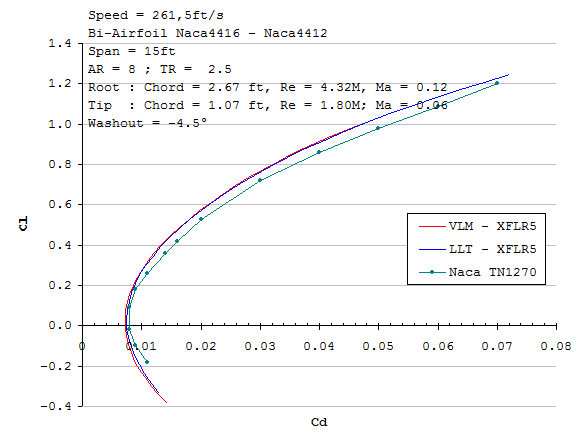
\includegraphics[width=0.8\linewidth]{img-36}\centering 
  \caption{Comparison to test results from Naca Tech. Note 1270}
  \label{fig:comparison_to_test_results}
\end{figure}


\subsubsection{Comparison to wind tunnel data}

An experiment has been carried out beginning of 2008 on a model
sailplane. The detailed results are given in \cite{DeperroisResults}.

The following figures provide results from XFLR5 v3.21 and from v4.09.
Results from v3.21 are marked as "FMe", since the calculation has
been performed by F. Meschia.

Note : in v4.09, the lift calculation was performed by integration of
pressure forces on the panels. From v4.13, the calculation is
performed in the far field plane.

\begin{figure}[htbp]
  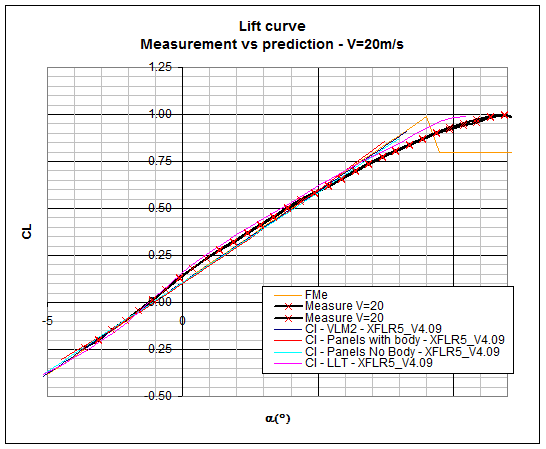
\includegraphics[width=0.8\linewidth]{img-37}\centering 
  \caption{Predicted lift curve vs. experimental results}
  \label{fig:predicted_lift_curve_vs_experimental_results}
\end{figure}

\begin{figure}[htbp]
  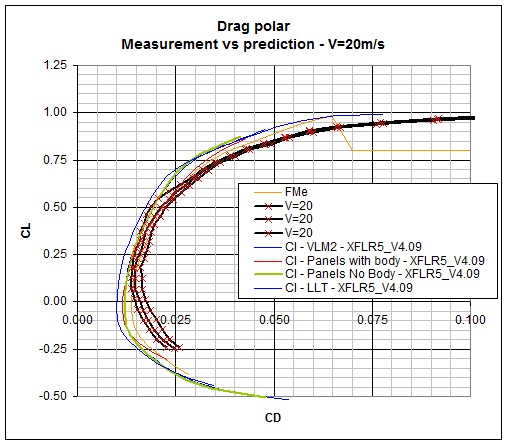
\includegraphics[width=0.8\linewidth]{img-38}\centering 
  \caption{Predicted drag polar vs. experimental results}
  \label{fig:predicted_drag_polar_vs_experimental_results}
\end{figure}

\begin{figure}[htbp]
  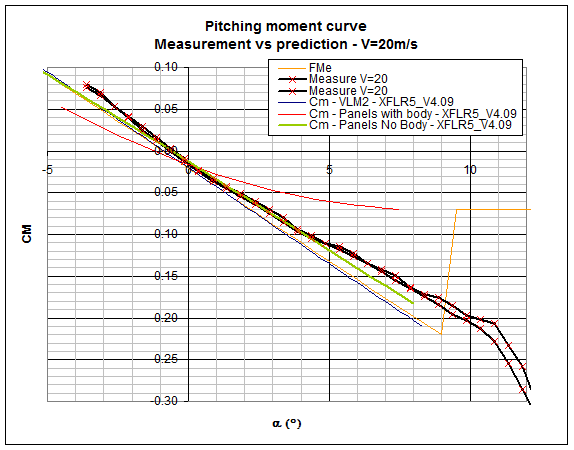
\includegraphics[width=0.8\linewidth]{img-39}\centering 
  \caption{Predicted pitch moment vs. experimental results}
  \label{fig:predicted_pitch_moment_vs_experimental_results}
\end{figure}

It can be concluded that

\begin{itemize}
\item the VLM is at least as reliable as the 3D panel method,
\item the body modeling does not improve the precision of the
results
\item both methods give reasonable estimations of values such
as :
\begin{itemize}
\item lift coefficient
\item zero lift angle
\item pitch moment coefficient
\item zero lift moment or zero moment lift
\end{itemize}
\item both methods tend to underestimate the drag, probably
the viscous part of it
\end{itemize}

\subsubsection{Comparison to Miarex and AVL results}

\begin{figure}[htbp]
  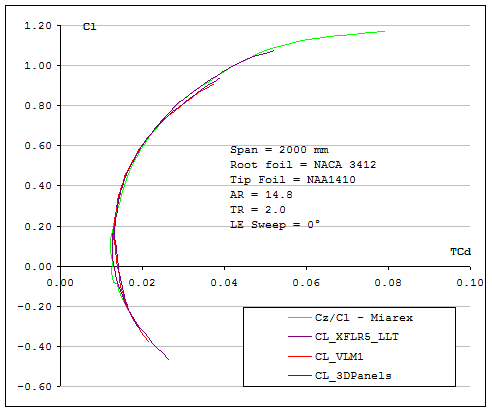
\includegraphics[width=0.8\linewidth]{img-40}\centering 
  \caption{Comparison to results from Miarex}
  \label{fig:comparison_to_results_from_miarex}
\end{figure}

\begin{figure}[htbp]
  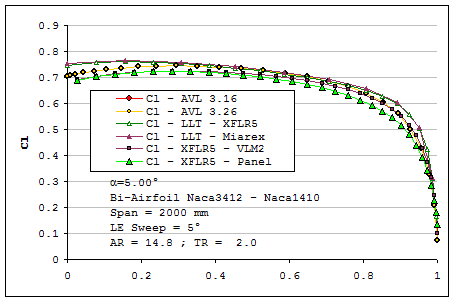
\includegraphics[width=0.8\linewidth]{img-41}\centering 
  \caption{Lift coefficient - Comparison to AVL and Miarex}
  \label{fig:lift_coefficient_comparison_to_avl_and_miarex}
\end{figure}

\begin{figure}[htbp]
  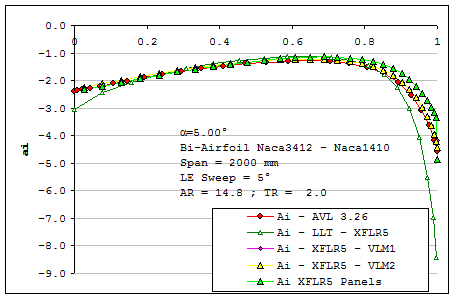
\includegraphics[width=0.8\linewidth]{img-42}\centering 
  \caption{Induced Angle vs. span - Comparison to AVL and Miarex}
  \label{fig:induced_angle_vs_span_comparison_to_avl_and_miarex}
\end{figure}

\begin{figure}[htbp]
  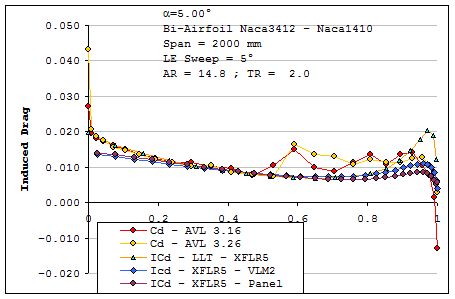
\includegraphics[width=0.8\linewidth]{img-43}\centering 
  \caption{Induced Drag vs. span - Comparison to AVL and Miarex}
  \label{fig:induced_drag_vs_span_comparison_to_avl_and_miarex}
\end{figure}

Note about induced drag : the heterogeneity of AVL results is
unexplained.

\begin{figure}[htbp]
  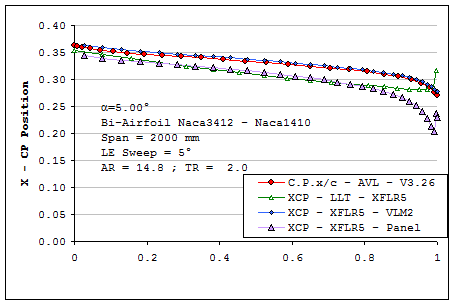
\includegraphics[width=0.8\linewidth]{img-44}\centering 
  \caption{Center of pressure position vs. span - Comparison to AVL and Miarex}
  \label{fig:center_of_pressure_position_vs_span_comparison_to_avl_and_miarex}
\end{figure}

\begin{figure}[htbp]
  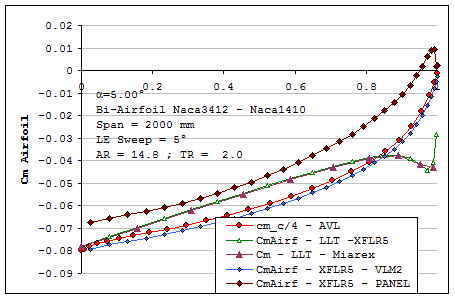
\includegraphics[width=0.8\linewidth]{img-45}\centering 
  \caption{Pitching moment coefficient vs. span - Comparison to AVL and Miarex}
  \label{fig:pitching_moment_coefficient_vs_span_comparison_to_avl_and_miarex}
\end{figure}

\subsubsection{Session example -- Wing Analysis}
\label{sec:session_example_wing_analysis}

\begin{enumerate}
\item Load the foil(s) which will be used to define the wing
\item In the Direct Analysis Application, click the "Run Batch
Analysis" command in the Polars menu, or type \Shift + \keystroke{F6}
\item Run a batch analysis with the following parameters (make sure these
values cover the whole flight envelope of the wing):
\begin{itemize}
\item from $\alpha = -6^\circ$ to $\alpha = 10^\circ$
\item from Re = 40,000 to Re = 160,000 every 20,000
\item from Re = 200,000 to Re = 500,000 every 50,000
\end{itemize}
or use a predefined list Checking the box "Start from zero" will cause
the analysis to start from $\varpi = 0^\circ$, going upwards to
$\alpha_{max}$, then downwards to $\alpha_{min}$ this usually
facilitates convergence
\item Close the dialog box
\item Optional : Use the "Save Associated Polars" in the "Current
Foil" menu to save the polars to a ".plr" file for use in future
projects
\item Switch to the Wing Design Application \Ctrl+\keystroke{6}
\item Click the"Define Wing" command, \keystroke{F3} in the Wing
menu, or "Define a Plane" (\Ctrl+\keystroke{F3})
\item Define the object and close the dialog box
\item Optional, but recommended : Define the inertia properties of the current
plane or wing object.
\item Select Current plane(or wing)/Define Inertia
\item Enter the inertia properties for the plane or wing.
\item Make sure that the CoG position is where it's meant to
be. It may be necessary to "cheat" a little
on the positions of point masses to achieve the desired position
\item Close the dialog box
\item Click the "Define Analysis/polar" in the
Wing Polar menu, (\keystroke{F6})
\item Activate the Type 2 check box
\item Define the plane mass and the center of gravity position (the moment
ref. location), or select the option to use the
plane's inertia
\item Unless the wing has either low aspect ratio, high sweep, or high
dihedral, select the"LLT" checkbox, and
close the dialog box (\Return and \Return)
\item Leave the LLT settings to the default values in the "Operating
Point" menu, i.e. "Relax~Factor~=~20" and
"$N^\circ$~of~Stations~Along~the~Span~=~20"
\item Select an angle of attack in the right toolbar which can be
expected to give positive lift equal to the model weight at reasonable
Speed/Re values -- for instance $\alpha = 3^\circ$
\item Click the"Analyze" button in the right toolbar
\item Change settings if LLT convergence cannot be reached, or
continue the LLT analysis after un-checking the "Init LLT" checkbox
\item Click the "3D view" command in the View menu
\item Use the mouse to zoom and rotate the model
\item Use Sequence to calculate a complete wing's polar
\item Click on the "Polars" command in the View
menu, (\keystroke{F8}) to visualize the
polar graphs
\end{enumerate}

\subsubsection{Non convergences}

\begin{table}[htbp]\scriptsize
  \centering
  \begin{tabular}{|m{0.18\linewidth}|m{0.38\linewidth}|m{0.38\linewidth}|}
    \hline
    &
    Cause &
    Fix \\
    \hline
    \multirow{4}{0.18\linewidth}{All methods} & 
    The foils' Type 1 polar meshes do not cover the available flight
    envelope\newline
    [most usual case of non convergence] &
    Extend the foils' Type 1 polar meshes \\
    \cline{2-3}
    &
    In Type 2 analysis, the lift is negative &
    Calculate only for higher values of the angle of attack \\
    \cline{2-3}
    &
    In Type 2 analysis, the speed is either too low or too high,
    leading to OpPoints outside of the available flight envelope &
    Extend the foils' Type 1 polar mesh ; The speed will tend towards
    infinite values at low aoa, and symmetrically will tend towards 0 at
    high aoa \\
    \cline{2-3}
    &
    The tip chord is too small and yields too low Reynolds numbers &
    Either: 
    \begin{enumerate}
    \item Check the "Store OpPoints outside the Polar mesh" checkbox
    \item Omit the end of the wing in the definition of its planform
    \end{enumerate} \\
    \hline
    \multirow{2}{0.18\linewidth}{LLT} & 
    The relaxation factor is too small &
    Increase the factor in the "LLT Settings…" dialog box \\
    \cline{2-3}
    &
    The number of points over the planform is too high &
    Decrease the number in the "LLT Settings…" dialog box \\
    \hline
    VLM &
    The matrix is singular because of a conflicting disposition of VLM panels &
    Regenerate a manual VLM mesh \\
    \hline
    Panel &
    The results are inconsistent because the wakes shedded by the wing
    and elevator are in the same horizontal plane &
    Offset either the wing or elevator in the z direction, so that they do not lie in the same plane \\
    \hline
  \end{tabular}
  \caption{Non convergences causes and solutions}
  \label{tab:non_convergences_causes_and_solutions}
\end{table}

The log file will indicate which points of the flight envelope could
not be calculated. It can be accessed with the menu command
"Operating Point/View Log File"

The "log file" is a plain text file. If the document does not show
up when called from the menu, it may be necessary to manually
associate the".log" extension to Windows' Notepad.


\subsection{Stability and control anaysis}

The intent of stability and control analysis is to evaluate the time
response of a plane to perturbations from a steady flight condition.
The perturbations can originate with the environment, for instance from
a gust of wind, or from the actuation of a control.

The mathematical representation of the response is a complex matter,
which requires some simplifying assumptions. Essentially, only small
perturbations about the steady flight conditions are considered.

The theoretical aspects of flight dynamics and stability analysis can be
found in reference \cite{Sivells47}. The purpose of this document is:

\begin{itemize}
\item to provide a short and much simplified description of
the flight dynamics for users not familiar with the theory
\item to explain the choices made in XFLR5
\item and to describe the analysis procedure.
\end{itemize}

Note : the mathematical concepts and formulas presented hereafter are
not absolutely necessary to the understanding of the physics of flight
dynamics. They are provided as information and background for those
users interested in investigating further the concepts.

\subsubsection{Method}

\subsubsection{Theory}

XFLR5 follows the method proposed by Etkin in ref [1].

With this type of analysis, longitudinal and lateral dynamics are
independent and are evaluated separately.

\subsubsection{Frames of reference}

Three different reference frames come into consideration in stability
analysis : the geometric axes, the body, axes and the stability axes.
These are defined in Figure~\ref{fig:body_and_stability_axes}.

\begin{figure}[htbp]
  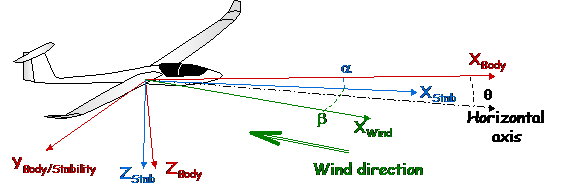
\includegraphics[width=0.8\linewidth]{img-46}\centering 
  \caption{Body and stability axes}
  \label{fig:body_and_stability_axes}
\end{figure}

\underline{Body axes:}

The term body axes is generic and refers to any frame which is fixed to
the body, and is therefore not an inertial frame of reference. A usual,
but not universal, convention is as follows:

\begin{itemize}
\item the X'-axis is aligned with the
fuselage nose;
\item the Z'-axis is in the plane of
symmetry, and points downwards;
\item the Y'-axis is perpendicular to the
XZ-plane and points starboard.
\end{itemize}

\underline{Geometric axes:}

This is the reference frame in which the geometry is defined.

\begin{itemize}
\item the X-axis is aligned
"backwards"
\item the Z-axis is in the plane of symmetry, and points
upwards;
\item the Y-axis is perpendicular to the xz-plane and points
starboard.
\end{itemize}

The geometric axes are a special case of body axes.

\underline{Stability axes:}

This is the frame in which the movement in the steady state conditions
is most conveniently described:

\begin{itemize}
\item the x-axis is the projection of the velocity vector on
the body's xz-plane; this axis therefore points
forward
\item the z-axis points downwards
\item the y-axis points starboard
\end{itemize}

The point of origin of the frame is the plane's centre
of gravity CoG.

The stability axes are a special case of body axes.

\underline{Notes:}

\begin{itemize}
\item In horizontal level flight, the axis
$X_{stability}$ is horizontal
\item Since sideslip in XFLR5 is simulated by rotation of the
structure around the inertial $Z_E$ axis, the wind axes
are the same as the stability axes even if the sideslip is non zero.
\item In equilibrium conditions, the stability axes are fixed
to the body, and therefore are not an inertial frame.
\end{itemize}

XFLR5 follows the recommendation of [1] and performs all calculations in
stability axes.

\subsubsection{Coordinates, position, velocity, and rotation vector}

The position of the body in stability axes is defined in some inertial
frame of reference by the position of its origin O(x,y,z), and by the
rotation defined by Euler angles (\textrm{${\varphi}$, ${\theta}$,
${\psi}$}).

Let V(U,V,W) be the body's velocity vector, and let
\textrm{${\omega}$}(P,Q,R) be the body's rotation
vector, both defined in the stability axes.

Additionally, assume that the plane is in equilibrium flight, for
instance :

\begin{itemize}
\item steady level flight with no sideslip
\item banked circle turn
\item looping at constant speed (difficult to imagine, but no
matter)
\end{itemize}

The state of the body/plane is defined by the set of variables (X, Y, Z,
U, V, W, P, Q, R)

Since we shall be considering only small variations about the steady
state conditions, each variable can be defined by an average value and
a perturbation around this mean value. For instance: \[U = U_0 + u\]

The subscript 0 refers to the steady flight state conditions.
$U_0$ for instance is the speed in level flight along the
stability x-axis.

The purpose of stability analysis is to calculate the time response of
the flight variables in response to small perturbations.

\subsubsection{Flight constraints}

The stability derivatives are computed about equilibrium conditions. The
conditions that are considered are level or banked horizontal flight.
Using terminology from AVL :

\begin{description}
\item[$\alpha$] angle of attack
\item[$\beta$] sideslip angle
\item[$C_L$] Lift coefficient, calculated from the geometry,
$\alpha$ and $\beta$.
\item[$\varphi$] arbitrary bank angle, positive to the right
\item[m] mass
\item[g] gravity acceleration
\item[$\varrho$] air density
\item[S] reference area
\end{description}

The constraints are :

\begin{itemize}
\item $U_0 = \sqrt{\frac{2mg}{\varrho SC_L} cos~\varphi}$ airspeed
\item $R_0 = \frac{V_0^2}{g}tan~\varphi$ turn radius, positive for right turn
\item $W_0 = \frac{V_0}{R}$ turn rate, positive for right turn
\item $p_0 = 0$ roll rate, zero for steady turn
\item $q_0 = W_0 sin~\varphi$ pitch rate, positive nose upward
\item $r_0 = W_0 cos~\varphi$ yaw rate, positive for right turn
\end{itemize}

Type 2 analysis in XFLR5 only considers the condition
\textrm{${\varphi}$}=0. This condition is relaxed for stability
analysis.

\subsubsection{State description}

The plane's state at any instant is given by a set of 8
variables. Four variables describe the longitudinal state:

\begin{description}
\item[u] is the variation of speed along the x-axis : $U = U_0 + u$
\item[w] is the variation of speed along the z-axis
\item[q] is the pitch rate, i.e. the rotation vector around the
y-axis
\item[$\theta$] is the pitch angle, i.e. the angle
between the stability x-axis and the horizontal flight line\newline
the angle is positive for a nose up.
\end{description}

Four variables describe the lateral dynamics:

\begin{description}
\item[v] is the variation of speed along the w-axis
\item[p] is the roll rate, i.e. the rotation vector around the x-axis
\item[r] is the yaw rate, i.e. the rotation vector around the z-axis
\item[$\varphi$] is the bank angle, i.e. the angle
between the stability y-axis and the horizontal flight line\newline
the angle is positive for a right wing down
\end{description}

The position defined by (x,y,z) does not come into consideration when
studying flight dynamics, since the behaviour is not expected to depend
on absolute position. The variation of gravity and density with
altitude is negligible for model aircraft and is not taken into
account.

In lateral dynamics, the heading \textrm{${\psi}$} does not appear in
the equations.

\subsubsection{Analysis procedure}

The stability analysis follows the following steps:

\begin{enumerate}
\item Define the geometry
\item Define the mass, center of gravity (CoG), and inertia of each component
of the plane. Two sub-options
\begin{enumerate}
\item Enter the mass of the wing or body, and let XFLR5 estimate the inertia
and CoG
\item Enter those values manually
\end{enumerate}
\item Define a stability Analysis/Polar (\Shift+\keystroke{F6}).\newline
If no active controls are defined, the analysis will be run for the base
geometry.\newline
If controls are defined, then the stability data may be calculated in a
sequence for a range of control parameter, and a polar curve may be
generated
\item Run the analysis for some control parameter. The code will
\begin{enumerate}
\item Search for an angle of attack such that Cm=0, and will exit with a
warning if unsuccessful
\item Calculate the trim speed to achieve steady state flight
\item Evaluate the stability derivatives,
\item Build the state matrices,
\item Extract the eigenvalues, and will exit with a warning if unsuccessful,
\item Store the data in an OpPoint (optional) and in the polar object.
\end{enumerate}
\item Visualize the results.
\end{enumerate}

\subsubsection{Input}

\paragraph{Description}

In input, the analysis takes :

\begin{itemize}
\item the plane's geometry
\item the plane's mass, CoG and inertia tensor, defined in geometrical
body axes.
\item the parameters defined by the stability analysis
\item the position for the controls : wing and elevator tilt angles,
flap positions, etc.
\item the type of steady flight to be considered : steady level flight
or steady banked turn.
\end{itemize}

\paragraph{Inertia estimations}

A calculation form is provided to evaluate approximately the CoG
position and the inertia tensor associated to the geometry. The
evaluation should not be understood as anything else than a rough
order of magnitude (ROM).

The inertia of the plane sums up the inertia of each object and of the
additional point masses.

\subparagraph{Object inertias}

The inertia of each object, i.e. wing or body, is evaluated in the
dialog form for this object. It includes the volume inertia from the
structural masses, and the inertia of point masses.

The volume inertia is evaluated based on the mass provided, and on the
geometrical data defining the object. It is evaluated in the
geometrical coordinate system, with origin at each object's CoG.

The evaluation is based on the following assumptions.

\begin{itemize}
\item For the body, the mass is distributed uniformly in the external
surface, and this surface is assumed to have a uniform thickness. The
body is divided in $N_b$ elementary sections along the x-axis. The
weight is concentrated at the center of the cross section, as
illustrated in Figure~\ref{fig:mass_representation_for_the_body}.
\item For the wing, the mass is assumed to be distributed uniformly in
the wing volume along the span.\newline
In XFLR5 v5, it has been modeled as point masses concentrated at the
quarter-chord point of distributed sections along the span.\newline
In XFLR5 v6, it is modeled as point masses distributed both in the
span and chord directions, as illustrated in
Figure~\ref{fig:mass_representation_for_the_wing}. The mass
distribution is independent of the wing's mesh used for aerodynamic
calculations.
\end{itemize}

\subparagraph{Point masses}

Parts such as actuators, battery, nose lead, or receiver should be
modelled separately as point masses, and not be included in the
evaluation of the volume inertia.

\subparagraph{Total inertia}

The total inertia for a plane is the sum of the inertias of the object
making up the plane, and of point masses. It is expressed in the
reference frame defined by the plane's CoG and by the geometrical
axes.

The transport of the inertia tensor from object CoG to plane CoG is
done by application of Huyghens/Steiner theorem.

\subparagraph{Notes}

\begin{itemize}
\item The mass defined for wings and bodies is not the one used for
Type 2 calculations. The mass for type 2 is defined by the
Analysis/Polar setting.
\item The distribution of point masses should be adjusted to obtain
the targeted position of the CoG. Otherwise, because of the
approximations made in the automatic evaluation of volume inertia, a
strict transposition of the "real" position of masses may result in
an incorrect position of the plane's CoG.
\end{itemize}

\begin{figure}[htbp]
  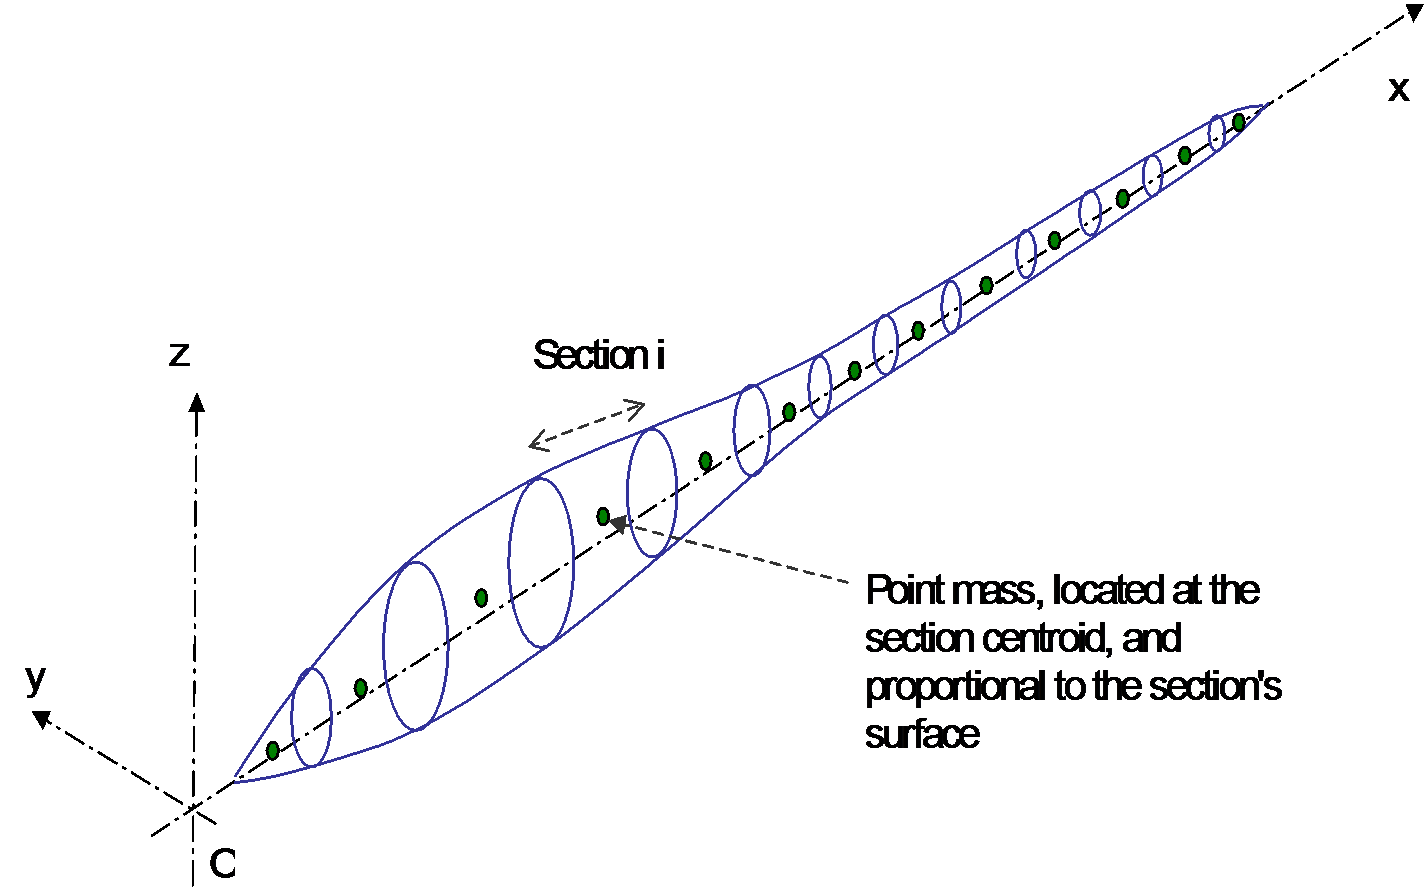
\includegraphics[width=0.8\linewidth]{img-47}\centering 
  \caption{Mass representation for the body}
  \label{fig:mass_representation_for_the_body}
\end{figure}

\begin{figure}[htbp]
  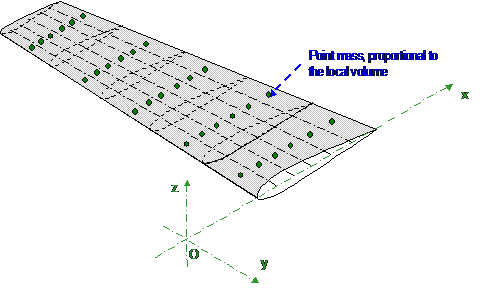
\includegraphics[width=0.8\linewidth]{img-48}\centering 
  \caption{Mass representation for the wing}
  \label{fig:mass_representation_for_the_wing}
\end{figure}

\paragraph{Stability polar parameters}

The"stability polars" replace the former "control polars". The
main difference is that the position of the CoG is no longer a
variable, but is instead determined by the distribution of masses in
the plane.

The Stability Polar object takes for input

\begin{itemize}
\item the fluid's density and dynamic viscosity
\item the type of reference length and area for the calculation of
aerodynamic parameters
\item the selection of either viscous or inviscid analysis
\item the control variables to include in the analysis
\end{itemize}

\paragraph{Control variables}

The polar points can be calculated for different state of control
variables. These variables are:

\begin{itemize}
\item The tilting of the wing about the y-axis
\item The tilting of the elevator about the y-axis
\item the rotation of the main wing's flaps about their hinge axis
\item the rotation of the elevator's flaps about their hinge axis
\item the rotation of the fin/rudder's flaps about their hinge axis
\end{itemize}


\underline{Notes:}

\begin{itemize}
\item The positive direction of rotation is positive by right-hand
rule, i.e.
\begin{itemize}
\item for the wing and elevator, a positive value will move the
leading edge upwards and the trailing edge downwards
\item for a wing or elevator flap, a positive control value will move
the trailing edge downwards
\item for the rudder, a positive control value will move the trailing
edge to starboard
\end{itemize}
\item To represent ailerons rotating in opposite directions, the min
and max values of the controls for each wing's aileron should be
opposite.
\item The initial value of the control's angle is not taken into
account in the analysis. For instance, if the flap has been defined
with foils with non-zero flap angles, the initial angles will be
cancelled before setting the position of the control.\newline
Similarly, the tilt angle defined for the wing or flap in the plane
definition is cancelled before application of the control variable.
\item For a control polar, all the parameters vary simultaneously in
accordance with the value of the control parameter "c" :
$$Control variable = (1-c) \times Control\_Min\_position + c \times Control\_Max\_position$$
\item The rotation of controls is not represented in the 3D view
\end{itemize}

\subsubsection{Output}

In output, the code provides results for longitudinal and lateral
dynamics :

\begin{itemize}
\item The dimensional stability and control derivatives
\item The non-dimensional stability derivatives
\item the time response for a step input
\item the eigenvalues and eigenvectors for the four longitudinal modes
and the four lateral modes.
\end{itemize}

\paragraph{Stability derivatives}

The stability derivatives describe the change to a force or moment in
response to a variation of a flight variable. For instance, the
variation of the axial force resulting from a change in axial speed
is:

$$\frac{\partial F_X}{\partial u} = 
\frac{1}{2}\rho \frac{\partial u_{0}^{2}} S C_X + 
\frac{1}{2}\rho u_{0}^{2} S \frac{\partial C_X}{\partial u}
= \rho u_{0} S C_{X} +
\frac{1}{2} \rho u_{0}^{2} S \frac{\partial C_{X}}{\partial u}$$

A usual convention is to use simplified notations:

$$\frac{\partial F_X}{\partial u} = X_u$$

$$\frac{\partial C_X}{\partial u} = Cx_u$$

with both derivatives being calculated in the steady state.

$X_u$ is the dimensional stability derivative, and
$Cx_u$ is the non-dimensional stability derivative.

XFLR5 calculates the dimensional derivatives which are relevant at the
scale of model sailplanes:

\begin{itemize}
\item In the longitudinal direction: $(X_u, X_w, Z_u, Z_w, Z_q, M_u, M_w, M_q)$
\item In the lateral direction: $(Y_v, Y_p, Y_r, L_v, L_p, L_r, N_v, N_p, N_r)$
\end{itemize}

The non-dimensional derivatives are usually given in stability axes, and
the derivatives w.r.t to v and w are provided instead w.r.t
$\alpha$ and $\beta$. They are :

\begin{itemize}
\item In the longitudinal direction $CL_a, CL_q, Cm_a, Cm_q$,
\item In the lateral direction : $CY_b, CY_p, CY_r, Cl_b, Cl_p, Cl_r, Cn_b, Cn_p, Cn_r$
\end{itemize}

The definition of the non dimensional derivatives is :

$$CLa = Zw \times u0  / (q \times S)$$

$$CLq = Zq \times 2. \times u0 / (q \times S \times mac)$$

$$Cma = Mw \times u0 / (q \times S \times mac)$$

$$Cmq = Mq \times (2. \times u0 / mac) / (q \times S \times mac)$$

$$CYb = Yv \times u0 / (q \times S)$$

$$CYp = Yp \times  2. \times u0 / (q \times S \times b)$$

$$CYr = Yr \times  2. \times u0 / (q \times S \times b)$$

$$Clb = Lv \times u0 / (q \times S \times b)$$

$$Clp = Lp \times (2. \times u0 / b) /(q \times S \times b)$$

$$Clr = Lr \times (2. \times u0 / b) /(q \times S \times b)$$

$$Cnb = Nv \times u0 / (q \times S \times b)$$

$$Cnp = Np \times (2. \times u0 / b) /(q \times S \times b)$$

$$Cnr = Nr \times (2. \times u0 / b) /(q \times S \times b)$$

Where :

\begin{itemize}
\item q is the dynamic pressure,
\item S is the reference Area
\item b is the reference Span
\item mac is the mean aerodynamic chord
\end{itemize}

The evaluation of the derivatives is an intermediate step in the
calculation of the dynamic response. The derivative values are stored
in the OpPoint object, and can be exported to a text file for use in
other flight simulation codes.

\paragraph{Modes}

\underline{Natural modes}

From the mathematical point of view, the state matrix can be
diagonalized for eigenvalues and eigenvectors. An eigenvalue is of the
form

$$\lambda = \sigma + i \omega $$

where

\begin{itemize}
\item $\sigma$ is the damping constant, unit 1/s
\item $\omega$ is the circular natural frequency, unit rad/s
\end{itemize}

Any eigenvalue with a non-zero imaginary part $\omega$, has a
symmetric eigenvalue given by the its conjugate. This implies that the
time response of a variable for such a mode is of the form :

$$x(t) = R e^{\sigma t} cos(\omega t - \varphi)$$

where $R$ and $\phi$ are constant values determined by the initial
conditions.

The mode will be dynamically stable if the damping is negative,
unstable otherwise. Dynamic stability means that when disturbed, the
plane will return progressively to its steady state flight.

Other definitions for oscillating modes : $ \omega_1=\sqrt{\lambda
\bar{\lambda}}=\sqrt{\sigma^2 + \omega^2}$ is the undamped natural
circular frequency, unit rad/s.

For damped modes, i.e. $ \sigma \textless 0$ , $\zeta =
\frac{-\sigma}{\omega_1}$ is the damping ratio, without unit :

\begin{itemize}
\item $\zeta \textgreater 1$ if the mode is overdamped
\item $\zeta = 1$ if the mode is critically damped
\item $\zeta \textless 1$ if the mode is underdamped, i.e.
oscillatory
\end{itemize}

If the damping is weak, i.e. $ \zeta^2 \textless \textless 1$, then $
\omega_1 \approx \omega$.

The frequency of vibration of the mode (unit Hz) is determined by :

$$F = \omega / 2 \pi $$

The time period (unit s) is :

$$T = 1 / F = 2 \pi / \omega $$

From the physics point of view, the eigenvalues and eigenvectors
represent the natural modes on which the plane will tend to oscillate.
For a standard well-defined problem, the modes will be:

\begin{itemize}
\item In the longitudinal case
\begin{itemize}
\item two symmetric phugoid modes
\item two symmetric short-period modes
\end{itemize}
\item In the lateral case
\begin{itemize}
\item a roll damping mode
\item a spiral mode
\item two symmetric dutch roll modes
\end{itemize}
\end{itemize}

\underline{Root Locus plot}

The position of the eigenvalues may be represented in the complex
plane, which is a convenient way to check visually the stability and
frequency of the modes :

\begin{itemize}
\item Roots (eigenvalues) lying on the left of the diagram with
negative x value correspond to stable modes, those lying on the right
with positive x-value are unstable.\newline
The further down the left is the root, the more stable is the mode.
\item Roots with non zero imaginary part correspond to oscillating
modes, those with zero imaginary part are non-oscillating.\newline
The further way is the root from the x-axis, the higher is the
frequency of vibration.
\end{itemize}

\underline{Mode shape}

The eigenvalue defines the mode's frequency and damping, and the
eigenvector defines its shape.

It isn't an intuitive task to understand a mode shape from the
eigenvector's components. Another more convenient way is to animate
the mode in the 3D view.

Since the frequency and damping may be very different from one mode to
the other, the time sampling and amplitude will need to be adjusted
for each mode.

The mode amplitude R is arbitrary and has no physical significance. It
may be adjusted to any scale for display purposes. In flight, a mode
is seldom excited alone. Rather, an external perturbation will tend to
generate a response on the different longitudinal and lateral modes.
This can be modelled in the time response plot.

\paragraph{Time response}

The time response is evaluated based on the flight dynamics equation.
For instance, in the longitudinal case, this is expressed as :

$$\left[\begin{matrix} \dot{u} \\ \dot{w} \\ \dot{q} \\ \dot{\theta} \end{matrix}\right] = \left[A_{long}\right] . \left[\begin{matrix} u \\ w \\  \\ \theta \end{matrix}\right] + \left[B_{long}\right] . \left[F(t)\right]$$

where:

\begin{itemize}
\item $\left[A_{long}\right]$ is the 4x4 longitudinal state matrix,
\item $\left[B_{long}\right]$ is the 4xn control influence matrix,
with n being the number of control variables
\item $\left[F(t)\right]$ is nx1 matrix, giving the forced input
history of each control variable
\end{itemize}

Similarly for lateral modes:

$$\left[\begin{matrix} \dot{v} \\ \dot{p} \\ \dot{r} \\ \dot{\varphi} \end{matrix}\right] = \left[A_{lat}\right] . \left[\begin{matrix} v \\ p \\ r \\ \varphi \end{matrix}\right] + \left[B_{lat}\right] . \left[F(t)\right]$$

The time history of the state variables (u, w, q, $\theta$)
and (v, p, r, $\varphi$) can be calculated either:
\begin{itemize}
\item as a consequence of perturbed initial conditions: this is
the "Initial condition response"
\item or as the consequence of control actuation vs. time : this is
the "Forced response"
\end{itemize}

\subparagraph{Initial condition response}

The input required is a step change from the steady state flight. For
the longitudinal case, this input may be provided as any combination
of values for u, w, and q. In the lateral case, it is input as a
combination of values of v, p, and r.

\subparagraph{Open loop forced response}

This type of analysis investigates the response of the plane to a
change of a control parameter. Such parameters are typically a
modification of thrust, or the actuation of a control surface such as
the elevator, the rudder, or the ailerons. The modification of thrust
is not considered in XFLR5.

The input required is a time history of a control parameter. XFLR5
only offers the possibility to simulate a linear ramp of a control in
a finite time.

\begin{figure}[htbp]
  \includegraphics[width=0.8\linewidth]{img-49}\centering 
  \caption{}
  \label{fig:}
\end{figure}

Although all control variables are set simultaneously to determine the
steady state geometry and trim conditions, the variation of each may
be set independently in the evaluation of the forced response. The
ramp time however is the same for all control variables.

Important note: the analysis of a response to a longitudinal step
input may have physical relevance since the plane may eventually
return to a steady state close to the initial conditions. On the
opposite, the actuation of lateral control will lead to divergence
from the steady state conditions, to coupling between longitudinal and
lateral modes, and the analysis will not be representative. For
instance, the ailerons will generate bank angle, modify the vertical
lift, and will lead to divergence from the steady state
conditions. The same goes for the actuation of the rudder, which will
lead for instance to bank angle through dihedral effect.

\subsubsection{Session example -- Stability analysis}

Run steps 1 through 8 as in the wing analysis session described in
\S\ref{sec:session_example_wing_analysis}.

\begin{enumerate}
\setcounter{enumi}{9}
\item Optional, but recommended : Define the inertia properties of the
current plane or wing object.
\begin{itemize}
\item Select Current plane (or wing) / Define Inertia
\item Enter the inertia properties for the plane or wing.
\item Make sure that the CoG position is where it's meant to be. It
may be necessary to "cheat" a little on the positions of point
masses to achieve the desired position
\item Close the dialog box
\end{itemize}
\item Optional : Click the "Define Analysis/Polar" in the Wing Polar
menu,
\begin{itemize}
\item select a type 1 or type 2 polar
\item Select "Use plane inertia", if previously defined
\item run a sequential analysis from low to high angles of attack
\item plot the graph $ICm=f(\alpha)$, make sure that the slope is negative
and that there is some a.o.a for which $ICm=0$
\end{itemize}
\item Click the "Define Stability Analysis" in the Wing Polar menu,
or type \Shift + \keystroke{F6}
\item Either decide to use the previously defined object inertia, or
input manually the mass, CoG position, and inertia properties
\item Optional : activate a control, and decide on the range of
variation
\item Close the dialog box (\Return and \Return). The polar's name
should now appear in the top middle combobox.
\item Select the control position in the right toolbar -- start with
0.  Deselect sequence.
\item Check the "Store OpPoint" checkbox
\item Click the "Analyze" button in the right toolbar
\item If the analysis has been successful, an OpPoint is automatically
added to the top right combobox. If not, check the log file to analyze
the error message.
\item In the polar view, check the "Show Point" checkbox for the
polar. In the $ICm=f(alpha)$ plot, the point should be located
precisely at the trimmed condiftion, i.e.  at the angle of attack for
which $ICm=0$
\item Switch to the stability analysis \Shift + \keystroke{F8}
\item Select either the root locus plot, or the time response view or
the 3D view
\end{enumerate}

Carry on to define a stability analysis with activated controls, and
view the stability properties as a function of control position.

\clearpage

\section{Code Specifics}

\subsection{XFoil, AVL and XFLR5}

XFLR5 has been developed based on XFoil V6.94. Later additions to
XFoil have not been included in XFLR5.

Since the algorithms have been re-written and integrated in XFLR5,
XFoil does not need to be present on the computer for XFLR5 to run. No
special links need to be declared.

XFLR5 does not use any of the AVL source code. The VLM algorithms have
been developed and implemented independently.

For AVL files generated by XFLR5, the foil's file names will need to
be checked, and it will also be necessary to check that the foil files
are present in the directory together with the other AVL files.

\subsection{Files and Registry}

Running XFLR5 will generate two files in the user's directory for
temporary files :

\begin{itemize}
\item "XFLR5.set" which records user settings ; delete this file to
restore the default settings
\item "XFLR5.log" which records the output of the foil and wing
analysis
\end{itemize}

The location of the directory is defined by the user's environment
variables.

XFLR5 itself does note write anything in the registry, but the
installation program will create shortcuts for the ".plr" and
".wpa" files. Users can choose to associate the foil ".dat" files
to XFLR5, but since this extension is used by Windows for many
different purposes, it has been deemed preferable to leave this choice
to the user.

Registry shortcuts will be removed by the uninstall process.

\subsection{Shortcuts}
In an attempt to increase the user friendliness of the interface,
shortcuts have been provided for most major commands, and are mentioned
in the menus.

Typing a first carriage return (\Return) in a dialog box will select
the OK or the default button, typing a second carriage return will
activate this button.

Typing a first carriage return (\Return) in the main window will
select the 'Analyze' button, typing a second carriage return will
activate this button.

\subsection{Mouse input}

All graphs, foils, and wings may be dragged and zoomed with the mouse.
Using \Ctrl + \LArrow button in 3D view will cause rotation of the model.

These options however may not work correctly (or not at all) if the
buttons are not set to the "Default" in the Windows Mouse interface.

Pressing the \keystroke{X} or \keystroke{Y} keys while zooming a graph
will expand only the corresponding axis.

For those computers without a mouse wheel nor a middle button, zooming
can be achieved in all views by pressing the \keystroke{Z} key and
moving the mouse.

\subsection{Memory}

One of the characteristics of both the foil and the wing analysis is
to use a significant computer memory.

Operating points specifically store a large amount of data and lead to
voluminous project files which will slow down Save \& Load processes.
It is however unnecessary to keep them, since the important data is
also stored in the polar objects which do not require large memory
resources.

\subsection{Export Options}

\underline{Printing}

Although XFLR5, as it is, offers some printing options, the
implementation of more advanced capabilities would require significant
work, and has not been, nor is expected to become, the primary concern
of the on-going development.

\underline{Screen Images}

An option has been added in v4.12 to export screen client areas to
image files.

\underline{Graph data}

An option has been added in v4.13 to export graph data to text files.

\underline{Data export}

All results, operating points and polars, can be exported to text
files for processing in a spreadsheet.

From v4.12 onwards, an option is available to export the data to the
"comma separated value" format ".csv". This text format is meant
to be readable without conversion in a spreadsheet. However, it may
happen that the operating system's regional settings need to be
adjusted to define the comma ',' as the default list separator.


\subsection{Bugs}

Once again, XFLR5 is by no means a professional program, and despite
the author's best efforts and the help of all those who have tested it
and provided valuable feedback, it is most probably still not
default-free.

Main Bug Corrections :

\begin{enumerate}
\item In the 3D panel method implemented in XFLR5 v4, the formulation for
Neumann boundary conditions was incorrect leading to inconsistent
results. For this reason, the default method has used Dirichlet
BC.\newline
The bug has been corrected in XFLR5 v6.02
\item A bug was reported shortly after the release of v3.00 on September
7\textsuperscript{th}, 2006. It had for main consequence to count twice
the elevator{\textquoteright}s lift in the calculation of a Plane with
the VLM quad-method. This bug has been corrected in version v3.01
released on September 24\textsuperscript{th}, 2006.
\item Up to v3.14, the contribution of the elevator and fin to the pitching
and yawing moments was calculated with respect to the point X=0 instead
of X=XCmRef. Corrected in v3.15 released January
21\textsuperscript{st}, 2007.
\end{enumerate}

The author will be grateful for any report of inconsistent results or
other bugs, and will do his best to investigate and correct them in a
timely manner. To facilitate bug corrections, the reports should
ideally include:

\begin{itemize}
\item The Operating System{\textquoteright}s identification (e.g. Windows XP
Pro, Vista{\dots})
\item The project file ("xxx.wpa")
\item The sequence of commands leading to the bug
\end{itemize}

\subsection{Open Source Development}

On March 31\textsuperscript{st}, 2007, XFLR5 has become an Open Source
Development Project hosted by
\href{http://sourceforge.net/projects/xflr5}{SourceForge.net}.

SourceForge provides a comprehensive set of tools and methods for a
project's development, and a documentation may be found
online. Potential contributors who would like to help organize the
project, correct bugs, or add new features and enhancements are
welcome.

\section{Credits}

Many thanks to Matthieu for his scientific advice and help, to Jean-Marc
for his patient and comprehensive testing of the preliminary versions,
to Marc for his natural ability to debug programs and planes, and to
all the others who have contributed by their input to improve XFLR5,
especially Giorgio and Jean-Luc.

Thanks also to Francesco who has written in RCSD 2008-04 a valuable
tutorial for XFLR5, and who has contributed to the development of the
version for MacOS

Similarly, thanks to Karoliina and Jean-Luc for her help in the
compilation of the Debian/Ubuntu version.

Thanks also to Martin for the German translation, and to Jean-Luc for
the French translation.

\clearpage

\section{References}

\begin{thebibliography}{99}

\bibitem{Sivells47} % [1]
  James C. Sivells and Robert H. Neely,
  \emph{Method for calculating wing characteristics by lifting line theory using nonlinear section lift data}.
  NACA Technical Note 1269,
  April 1947.

\bibitem{Neely} % [2]
  Robert H. Neely, Thomas V. Bollech, Gertrude C. Westrick, Robert R. Graham
  \emph{Experimental and calculated characteristics of several NACA-44 series wings with aspect ratios of 8, 10 and 12 and taper ratios of 2.5 and 3.5}.
  NACA Technical Note 1270.

\bibitem{Katz} % [3] 
  Katz \& Plotkin, 
  \emph{Low Speed Aerodynamics, From wing theory to panel methods}.
  Cambridge University Press, 2\textsuperscript{nd} Ed.,
  2001.

\bibitem{Maskew} % [4] 
  Brian Maskew,
  \emph{Program VSAERO Theory Document}.
  NASA Contractor Report 4023,
  September 1987.

\bibitem{Werner} % [5] 
  Sophia Werner,
  \emph{Application of the Vortex Lattice Method to Yacht Sails}.
  Master Thesis,
  July 200.

\bibitem{DeperroisStab} % [6] 
  André Deperrois,
  \emph{About stability analysis using XFLR5}
  Presentation document,
  June 2008,
  \url{http://xflr5.sourceforge.net/docs/XFLR5_and_Stability_analysis.pdf}.

\bibitem{DeperroisNotions} % [7]
  André Deperrois,
  \emph{Quelques notions d'a\'erodynamique de base et leur calcul dans XFLR5}
  Presentation document,
  June 2008,
  \url{http://xflr5.sourceforge.net/docs/Survol_Bases_Aero_et_XFLR5.pdf}.

\bibitem{DeperroisCtrlPolar} % [8]
  André Deperrois,
  \emph{Illustration of the use of Control Polars in XFLR5}
  Presentation document,
  July 2008,
  \url{http://xflr5.sourceforge.net/docs/Control_analysis.pdf}.

\bibitem{DeperroisResults} % [9]
  André Deperrois,
  \emph{Results vs. prediction}
  Presentation document,
  July 2008,
  \url{http://xflr5.sourceforge.net/docs/Results_vs_Prediction.pdf}.

\bibitem{Drela} % [10]
  Mark Drela \& Harold Youngren,
  \emph{Athena Vortex Lattice (AVL)}.
  \url{http://web.mit.edu/drela/Public/web/avl/}

\bibitem{Etkin} % [11]
  B. Etkin and L.D. Reid\
  \emph{Dynamics of Flight: Stability and Control}.
  John Wiley and Sons, New York, NY, Third Edition, 
  1996.

\bibitem{Deperrois2010} % [12]
  André Deperrois,
  \emph{Stability and Control analysis in XFLR5 v6}.
  Presentation document,
  September 2010,
  \url{http://xflr5.sourceforge.net/docs/XFLR5_and_Stability_analysis.pdf}.

\end{thebibliography}

\end{document}
